
\documentclass[a4paper,12pt]{article}
\usepackage{blindtext}
\usepackage[utf8]{inputenc}
\usepackage{graphicx}
\usepackage{enumitem}
\usepackage{booktabs}
\usepackage{verbatim}
\usepackage{makecell}
\usepackage[section]{placeins}
\usepackage{hyperref}
\usepackage[margin=1in]{geometry}

\usepackage{fancyhdr}

\pagestyle{fancy}
\fancyhf{}
\fancyhead[L]{User Manual}
\fancyhead[C]{}
\fancyhead[R]{}
\renewcommand{\headrulewidth}{0.4pt}
\fancyfoot[L]{Code 9}
\fancyfoot[C]{}
\fancyfoot[R]{Page \thepage}
\renewcommand{\footrulewidth}{0.4pt}


\begin{document}
	\begin{center}\thispagestyle{empty}
		
\includegraphics{Graphics/uplogo.jpg}
		
		{\Huge 
			2017 COS 301 Project \linebreak
			User Manual \linebreak 
			\par}
		
		{\Huge
			TEAM CODE 9
			\linebreak
			\par}
		
		\begin{LARGE}
			Seonin David
			\linebreak
			\linebreak
			Joshua Moodley
			\linebreak
			\linebreak
			Jaques Smulders
			\linebreak
			\linebreak
			Jordan Daubinet
			\linebreak
			\linebreak
			Nicaedin Suklul
		\end{LARGE}
	\end{center}
	
	\begin{figure}[b]
		\centering
		
\includegraphics[width=8cm]{Graphics/kpmgLogo.jpg}
	\end{figure}
\newpage
\tableofcontents
\newpage

\section{Introduction}
	This is the user manual for installing and setting up the project management system for KPMG.This manual contains instructions on how to download and install the server and database. This manual will also give you a basic understanding for how to create new employees and create projects.\linebreak\linebreak\textbf{This manual will currently not show you how to use the entire system because the system is still in pre-alpha}
\section{Installation}
\subsection{Inststalling MongoDB}
	\begin{itemize}
		\item Go to \url{ https://www.mongodb.com/download-center#community} and download MongoDB for your respective operating system.
		\item Install MongoDB (It will probably be installed in PoogramFiles/Mongo)
	\end{itemize}
\subsection{Starting MongoDB}
	\subsubsection{For Windows}
		\begin{itemize}
			\item Open command prompt
			\item Type \textit{cd /}
			\item Then navigate to the bin folder in the Mongo folder \linebreak (usually is \textit{cd C:/Program Files/MongoDB/Server/3.2/bin})
			\item Type \textit{mongod}. MongoDB will now be running.
			\item \textbf{Since our system is in pre-alpha we do not have an importable database as we are still doing testing and the database still contains dummy data therefore the DB you will be using is empty.}
		\end{itemize}
	
\newpage
\subsection{Installing NodeJS}
\begin{itemize}
	\item GO to \url{https://nodejs.org/en/download/} and download NodeJS for your respective operating system.
	\item Install NodeJS
\end{itemize}

	\subsection{Installing dependencies}
		\begin{itemize}
			\item Go to \url{https://github.com/Code9Developers/Back-End} and click on the\textbf{ Clone or Download } button, then click download ZIP to donwnload our repo.
			
			\item Unzip the repo and place it in a location that you would like to keep the system.
			
			\item Open command propmt (assuming windows) and navigate to the reopo until you in the folder with the package.json
			
			\item Then type \textit{npm install}. This will install all the packages required to run the system.
		\end{itemize}
		\subsection{Starting the server}
			\begin{itemize}
			\item After all the packages are installed, type \textbf{\textit{npm run dev}}.This will start the server (assuming MongoDB is still running).
			
			\item The server will now let you now that it is connected to the database and you can access the website on port 4000.
			
			\item To access the website type \textbf{\textit{https://localhost:4000}}
		\end{itemize}
\newpage

\section{Using the System}
The system is currently still in development but the core functionality can still be used.\textbf{Note that the routing authentication has been turned off, this is due to testing purposes but the functionality is there}

	\subsection{Login page}
	\begin{enumerate}
		\item Request type: GET
		\item URL: \url{https://localhost:4000/login} or \url{https://localhost:4000}
	\end{enumerate}

	\begin{flushleft}
			This is the login page where a manager,administrator or employee can login and will be routed to the relevant page.When the respective user logs in it will route to the respective page depending on that users role.
			\begin{enumerate}
    		\item Project Manager: Project creation page
    		\item Administrator: All employees page
    		\item Employee: User dashboard page
    	\end{enumerate}
	\end{flushleft}

    \subsection{Admin pages(If an administrator logs in)}
     	\subsubsection{Admin Page}
     		\begin{enumerate}
     		\item Request type: GET
     		\item URL:\url{https://localhost:4000/admin} 
     	\end{enumerate}
     	 \textbf{Description}
     	\begin{flushleft}
     		On this page an Admin user will be allowed to create a new employee with all the relevant information. Once submit button is clicked a POST request will be sent to the server, the employee will then be stored in the users collection in the database. 
     		
     		When you click on the submit button it will create the project and then route the logged in user to the employees page which will display all employees on the KPMG system.
     	\end{flushleft}
 		\textbf{Functions}
 		\begin{flushleft}
 			On this page when the submit button is clicked it will send a request to store all the information in the page. The employee that is created will then be stored in the database and now can be assigned to a project.After that the page will then route to the employees page(\url{https://localhost:4000/employees}) which will display all employees that are registered.
 		\end{flushleft}
 		\linebreak
 	    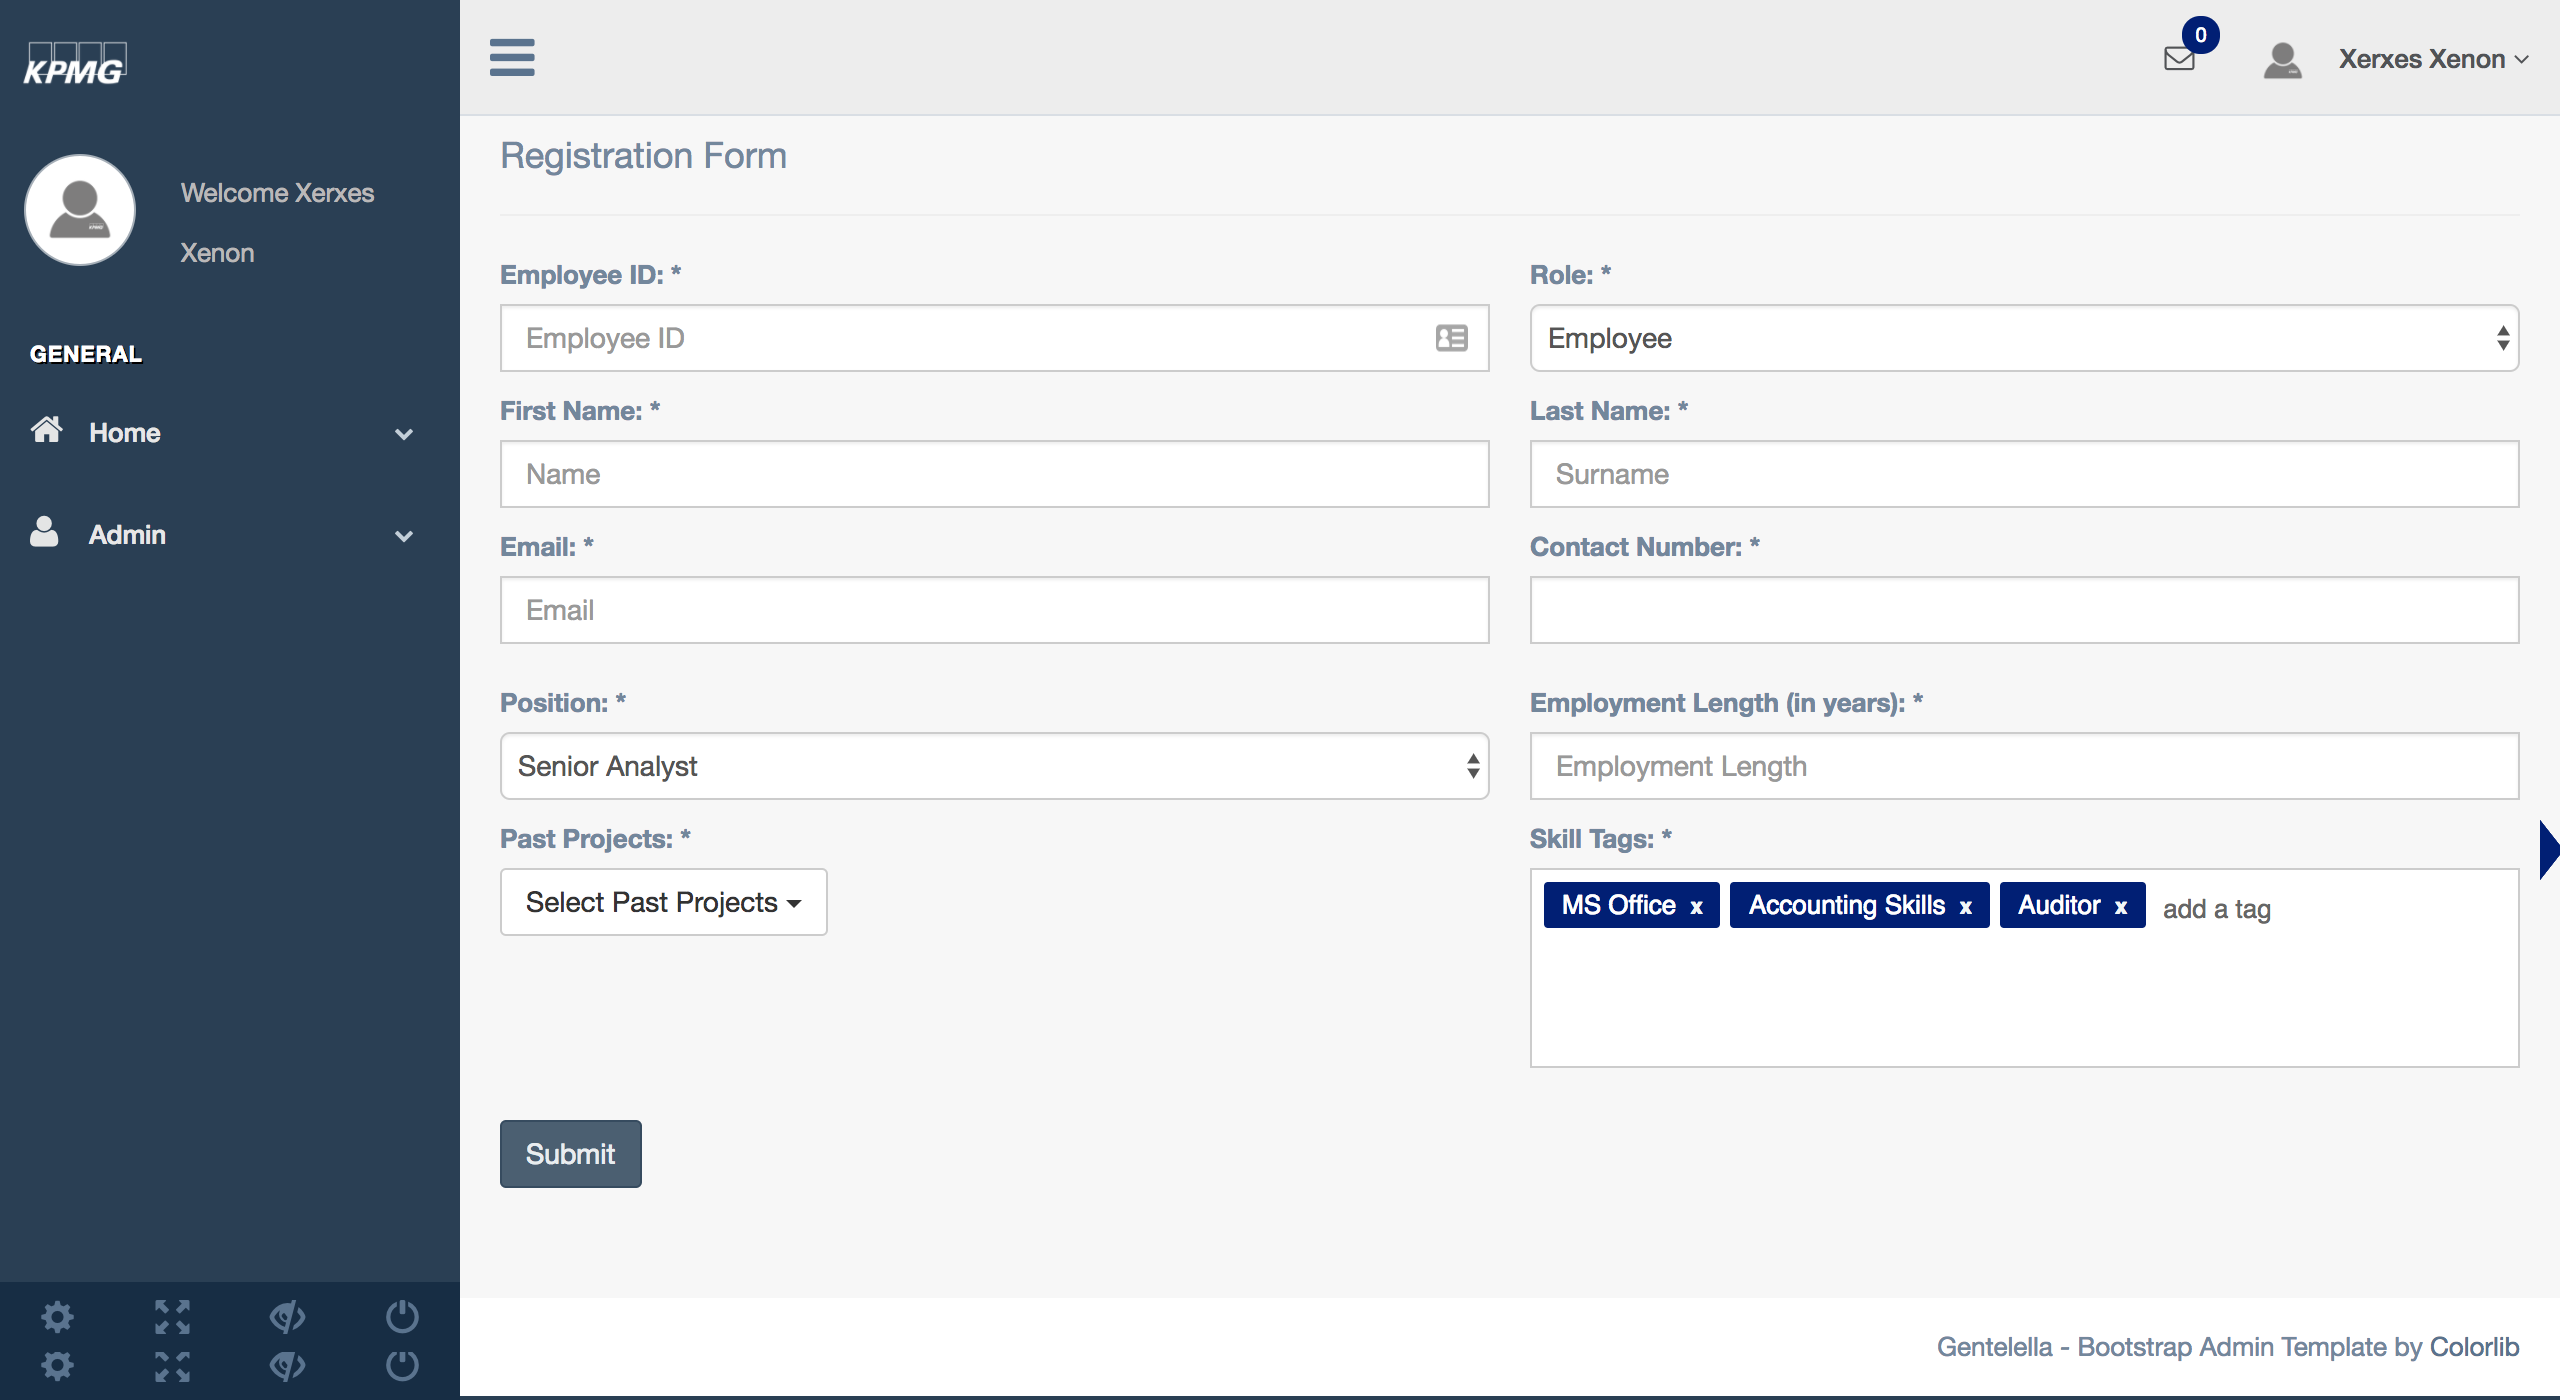
\includegraphics[width=0.99\linewidth]{Images/admin_register_emp.png}
 	\subsubsection{Employees Page}
	 	\begin{enumerate}
	 		\item Request type: GET
	 		\item URL:\url{https://localhost:4000/employees} 
	 	\end{enumerate}
 	\textbf{Description}
	 	\begin{flushleft}
	 		This page displays all the registered employees on the system.
	 	\end{flushleft}
 	\textbf{Functions}
		 \begin{flushleft}
		 	When the page loads it will call a function to get all the employee that are currently stored on the system.
		 	The administrator can click the view button and it will then route to the employees profile page where all the employees information can be seen.
		 \end{flushleft}
	  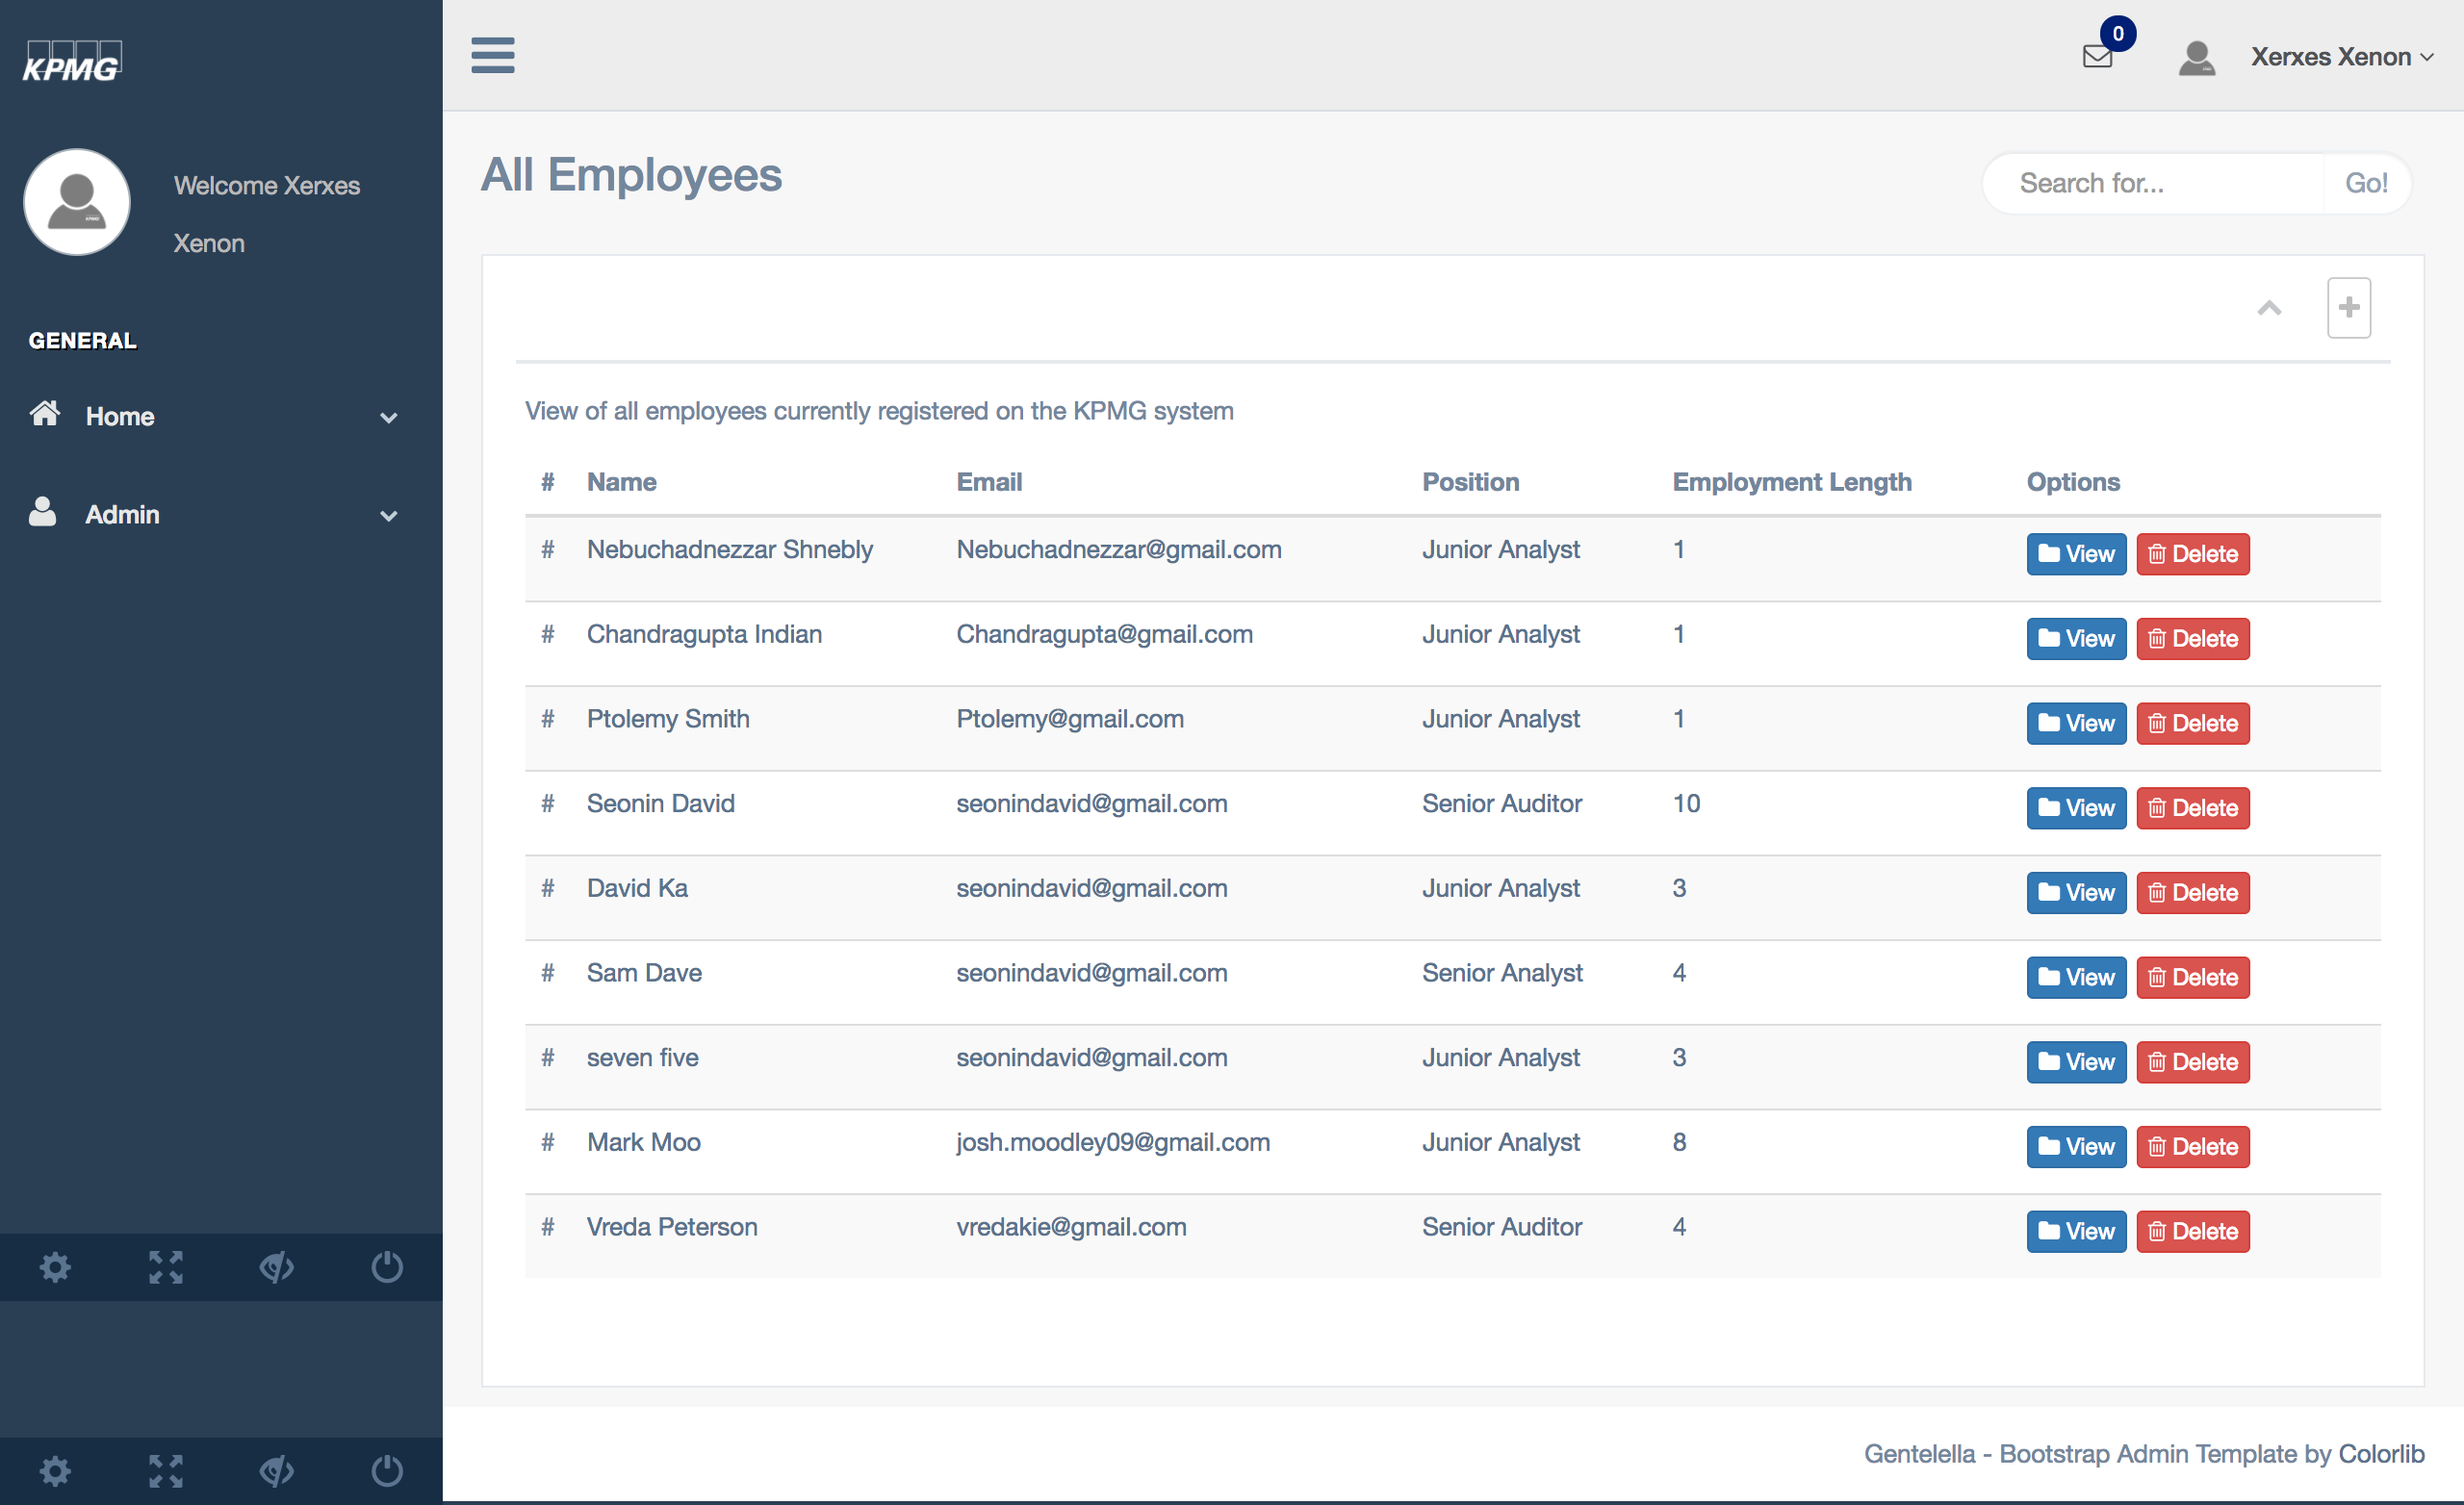
\includegraphics[width=0.99\linewidth]{Images/admin_dash.png}
	  
	  
	\subsection{Project pages (If a project manager logs in)}
		 \subsubsection{Project Creation Page}
		 		\begin{enumerate}
				 	\item Request type: GET
				 	\item URL: \url{https://localhost:4000/project_creation}
				 \end{enumerate}
				
				\textbf{Description}
				\begin{flushleft}
					On this page a manager can create the project.The manager will be required to enter all information relevant to the project. The manager will also have to select the number of employees that is required for the project.When the allocate employees button is clicked, the algorithm will then return the best suited employees for the project after taking many factors into account. The manager can then choose to remove employees from the project but this will have to go through the chain of command to get approved.After all the information is entered and the employees are selected. A POST request will then be sent to the server to store all the information in the database. After all the information is store the user will then be routed to the project view page where he/she can view all information regarding the project as well as insert information regarding the project.
				\end{flushleft}
			
			\textbf{Functions}
			\begin{flushleft}
				On this page when the employee clicks on the assign employees button a request for employees will be sent to the server. The server will then call the resource allocation algorithm to get the best suited employees and then return and display in the table.
				
				When the project manager clicks on the  
			\end{flushleft}
			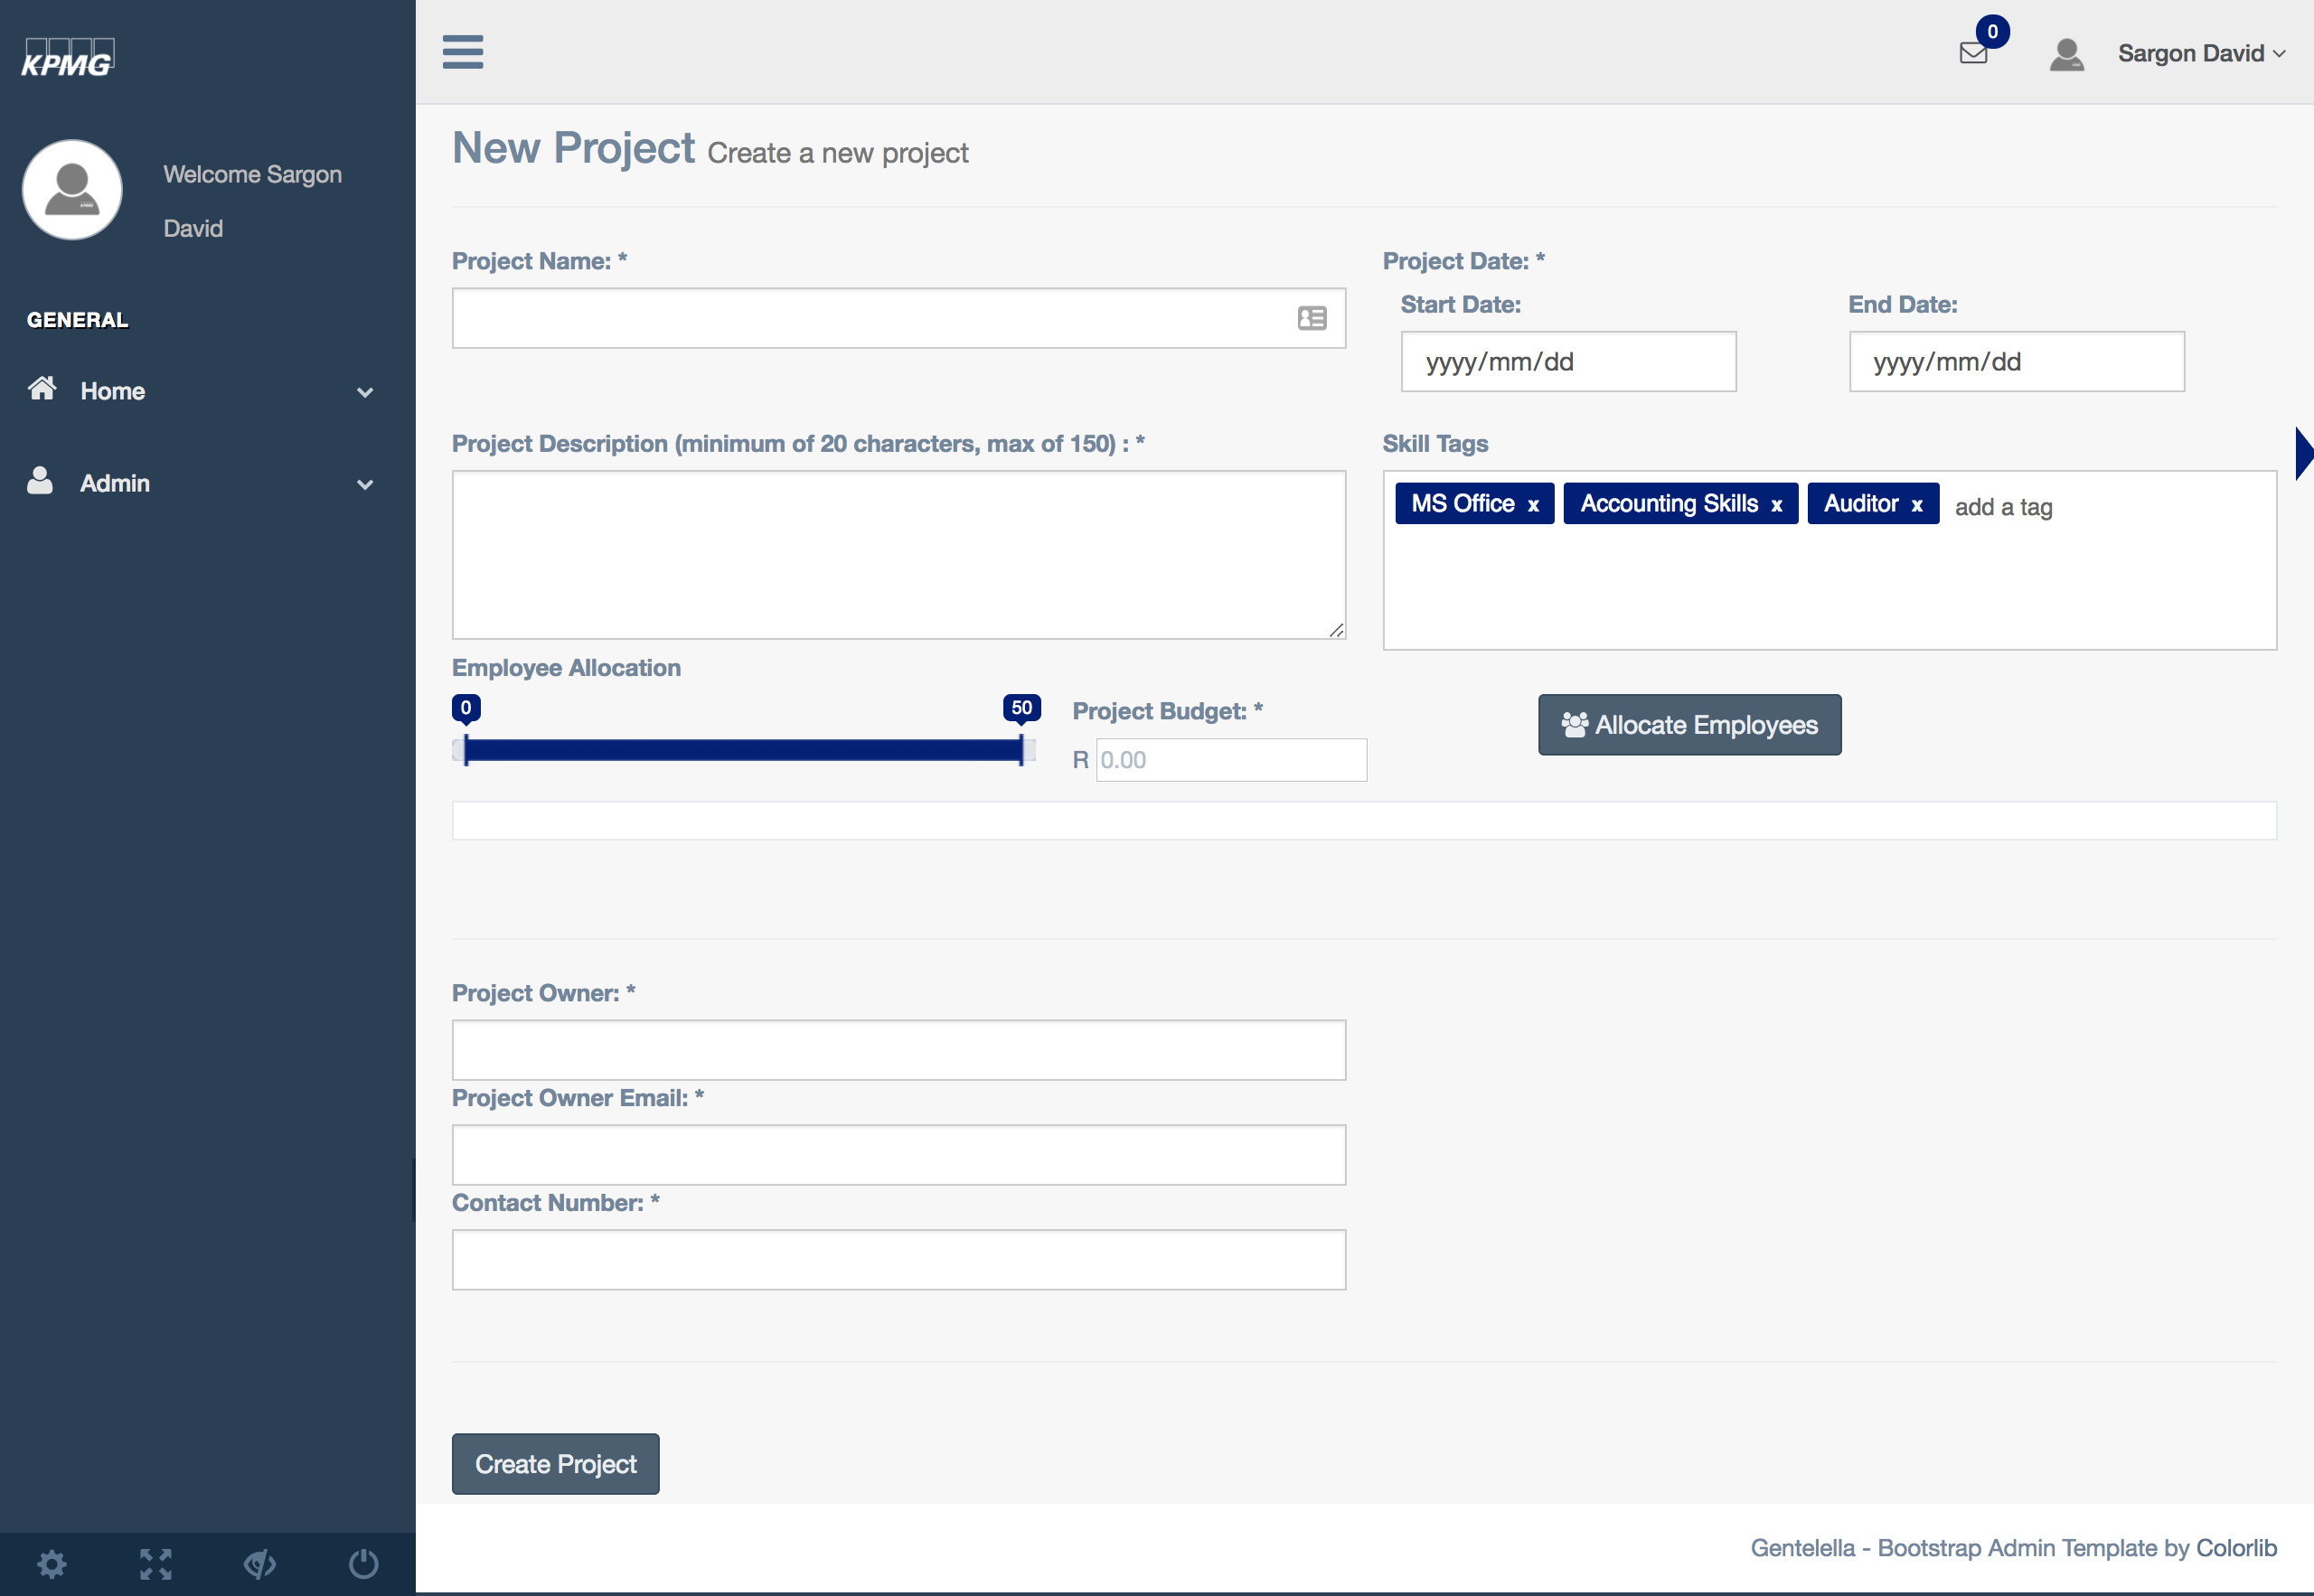
\includegraphics[width=0.99\linewidth]{Images/manager_create_project.png}
	  
			
		\subsubsection{Projects Page}
		 		\begin{enumerate}
				 	\item Request type: GET
				 	\item URL: \url{https://localhost:4000/projects}
				 \end{enumerate}
				
				\textbf{Description}
				\begin{flushleft}
				    This page displays all the projects that are currently active.From this page a project manager will be able to view the active projects as well as some brief details about the project such as date created and project start date.At the far left of the page there are four buttons, each button routes to the page to do the functionality described by the button.
				\end{flushleft}
				
				\textbf{Functions}
				\begin{flushleft}
				    \begin{enumerate}
				    	\item \textbf{Click View Button}- When this button is clicked it will send a GET request to the server to display the project view page of the project that was clicked(It sends the project ID in the get request so it only displays the appropriate project.)
				 	    \item \textbf{Click Milestones Button}- This button will route the manager to the milestones page where the manager can can add milestones to the project.
				 	    \item \textbf{Click Edit Button}- This page will route the manager to the project edit page where the manager can edit parts of the project.
				     \end{enumerate}
				\end{flushleft}
        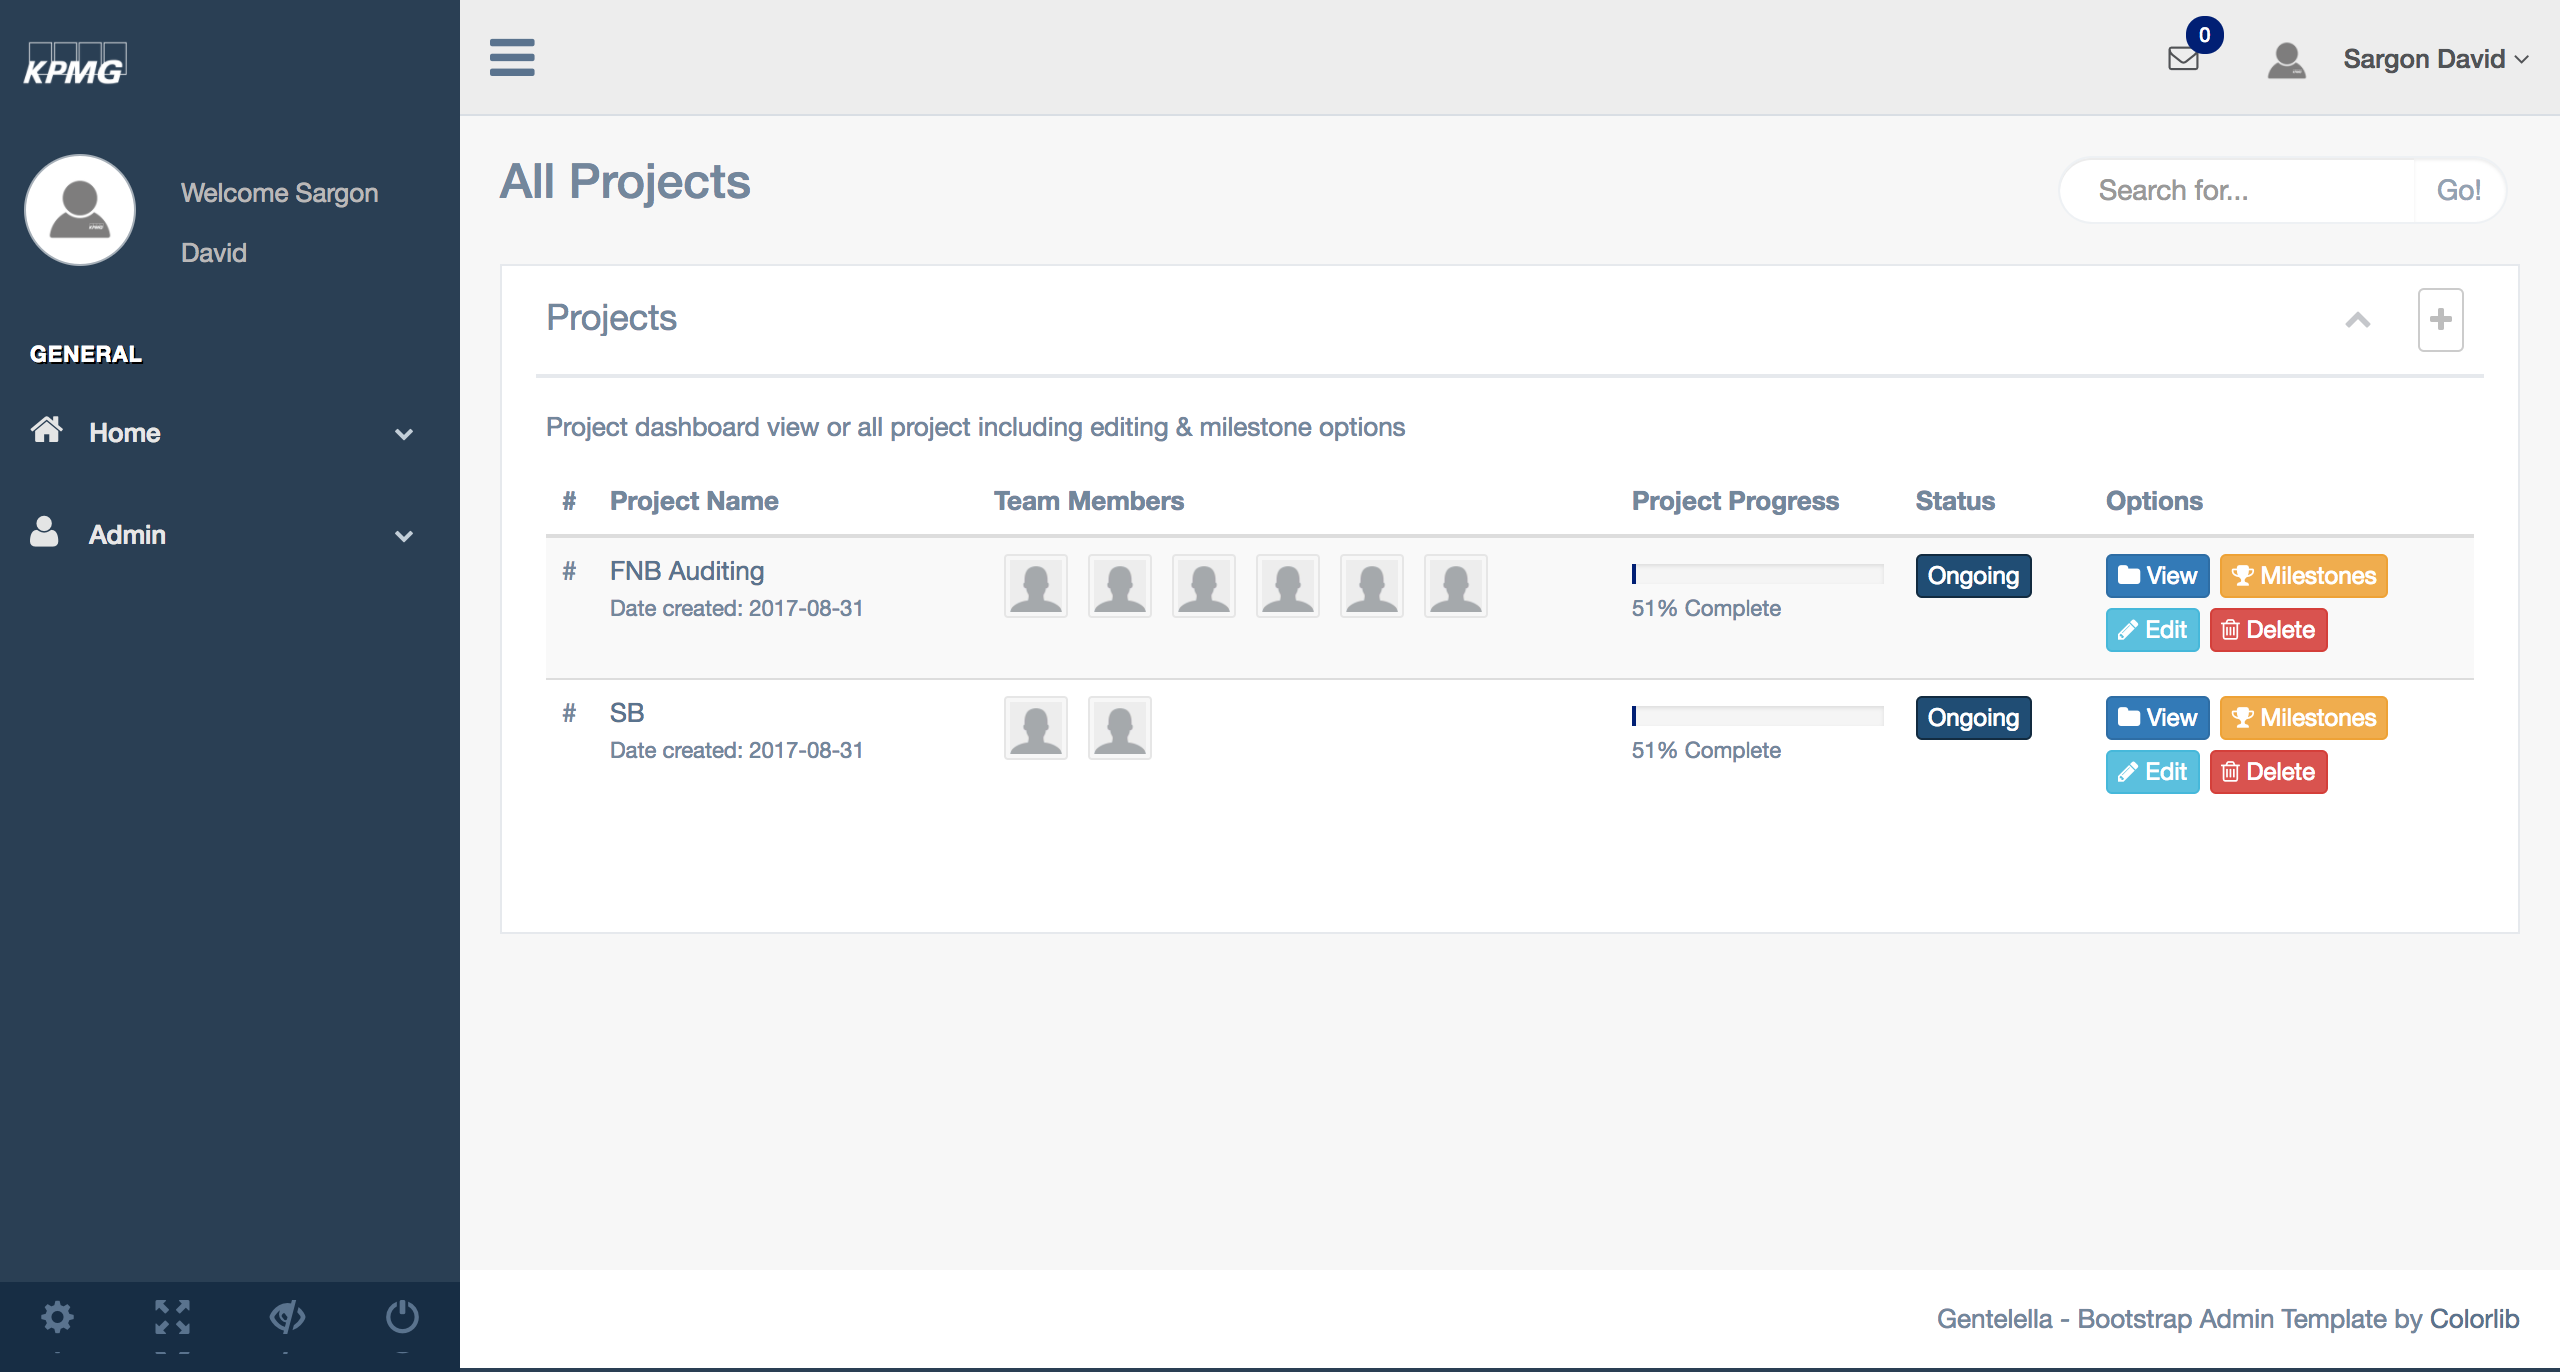
\includegraphics[width=0.99\linewidth]{Images/manager_project_dash.png}
        
        
        \subsubsection{Projects View}
		 		\begin{enumerate}
				 	\item Request type: GET
				 	\item URL: \url{https://localhost:4000/project_detail}
				 \end{enumerate}
				
				\textbf{Description}
				\begin{flushright}
				  This page displays all information about the project.The project manager can all create tasks at the bottom of the page.A manager can create as task assign it to a milestone and also assign it to multiple employees to finish.When a task is created an employee will get notified. When the task is complete the manager can just check it and it will move to the complete list.
				\end{flushright}
				
				\textbf{Functions}
				\begin{flushright}
				    \begin{enumerate}
				    	\item Allow manager to create task.This request will be sent to the server where the task and all relevant details associated with the task will get stored in the database, after that is done notifications will be created and relevant parties will be notified.
				     \end{enumerate}
				\end{flushright}
				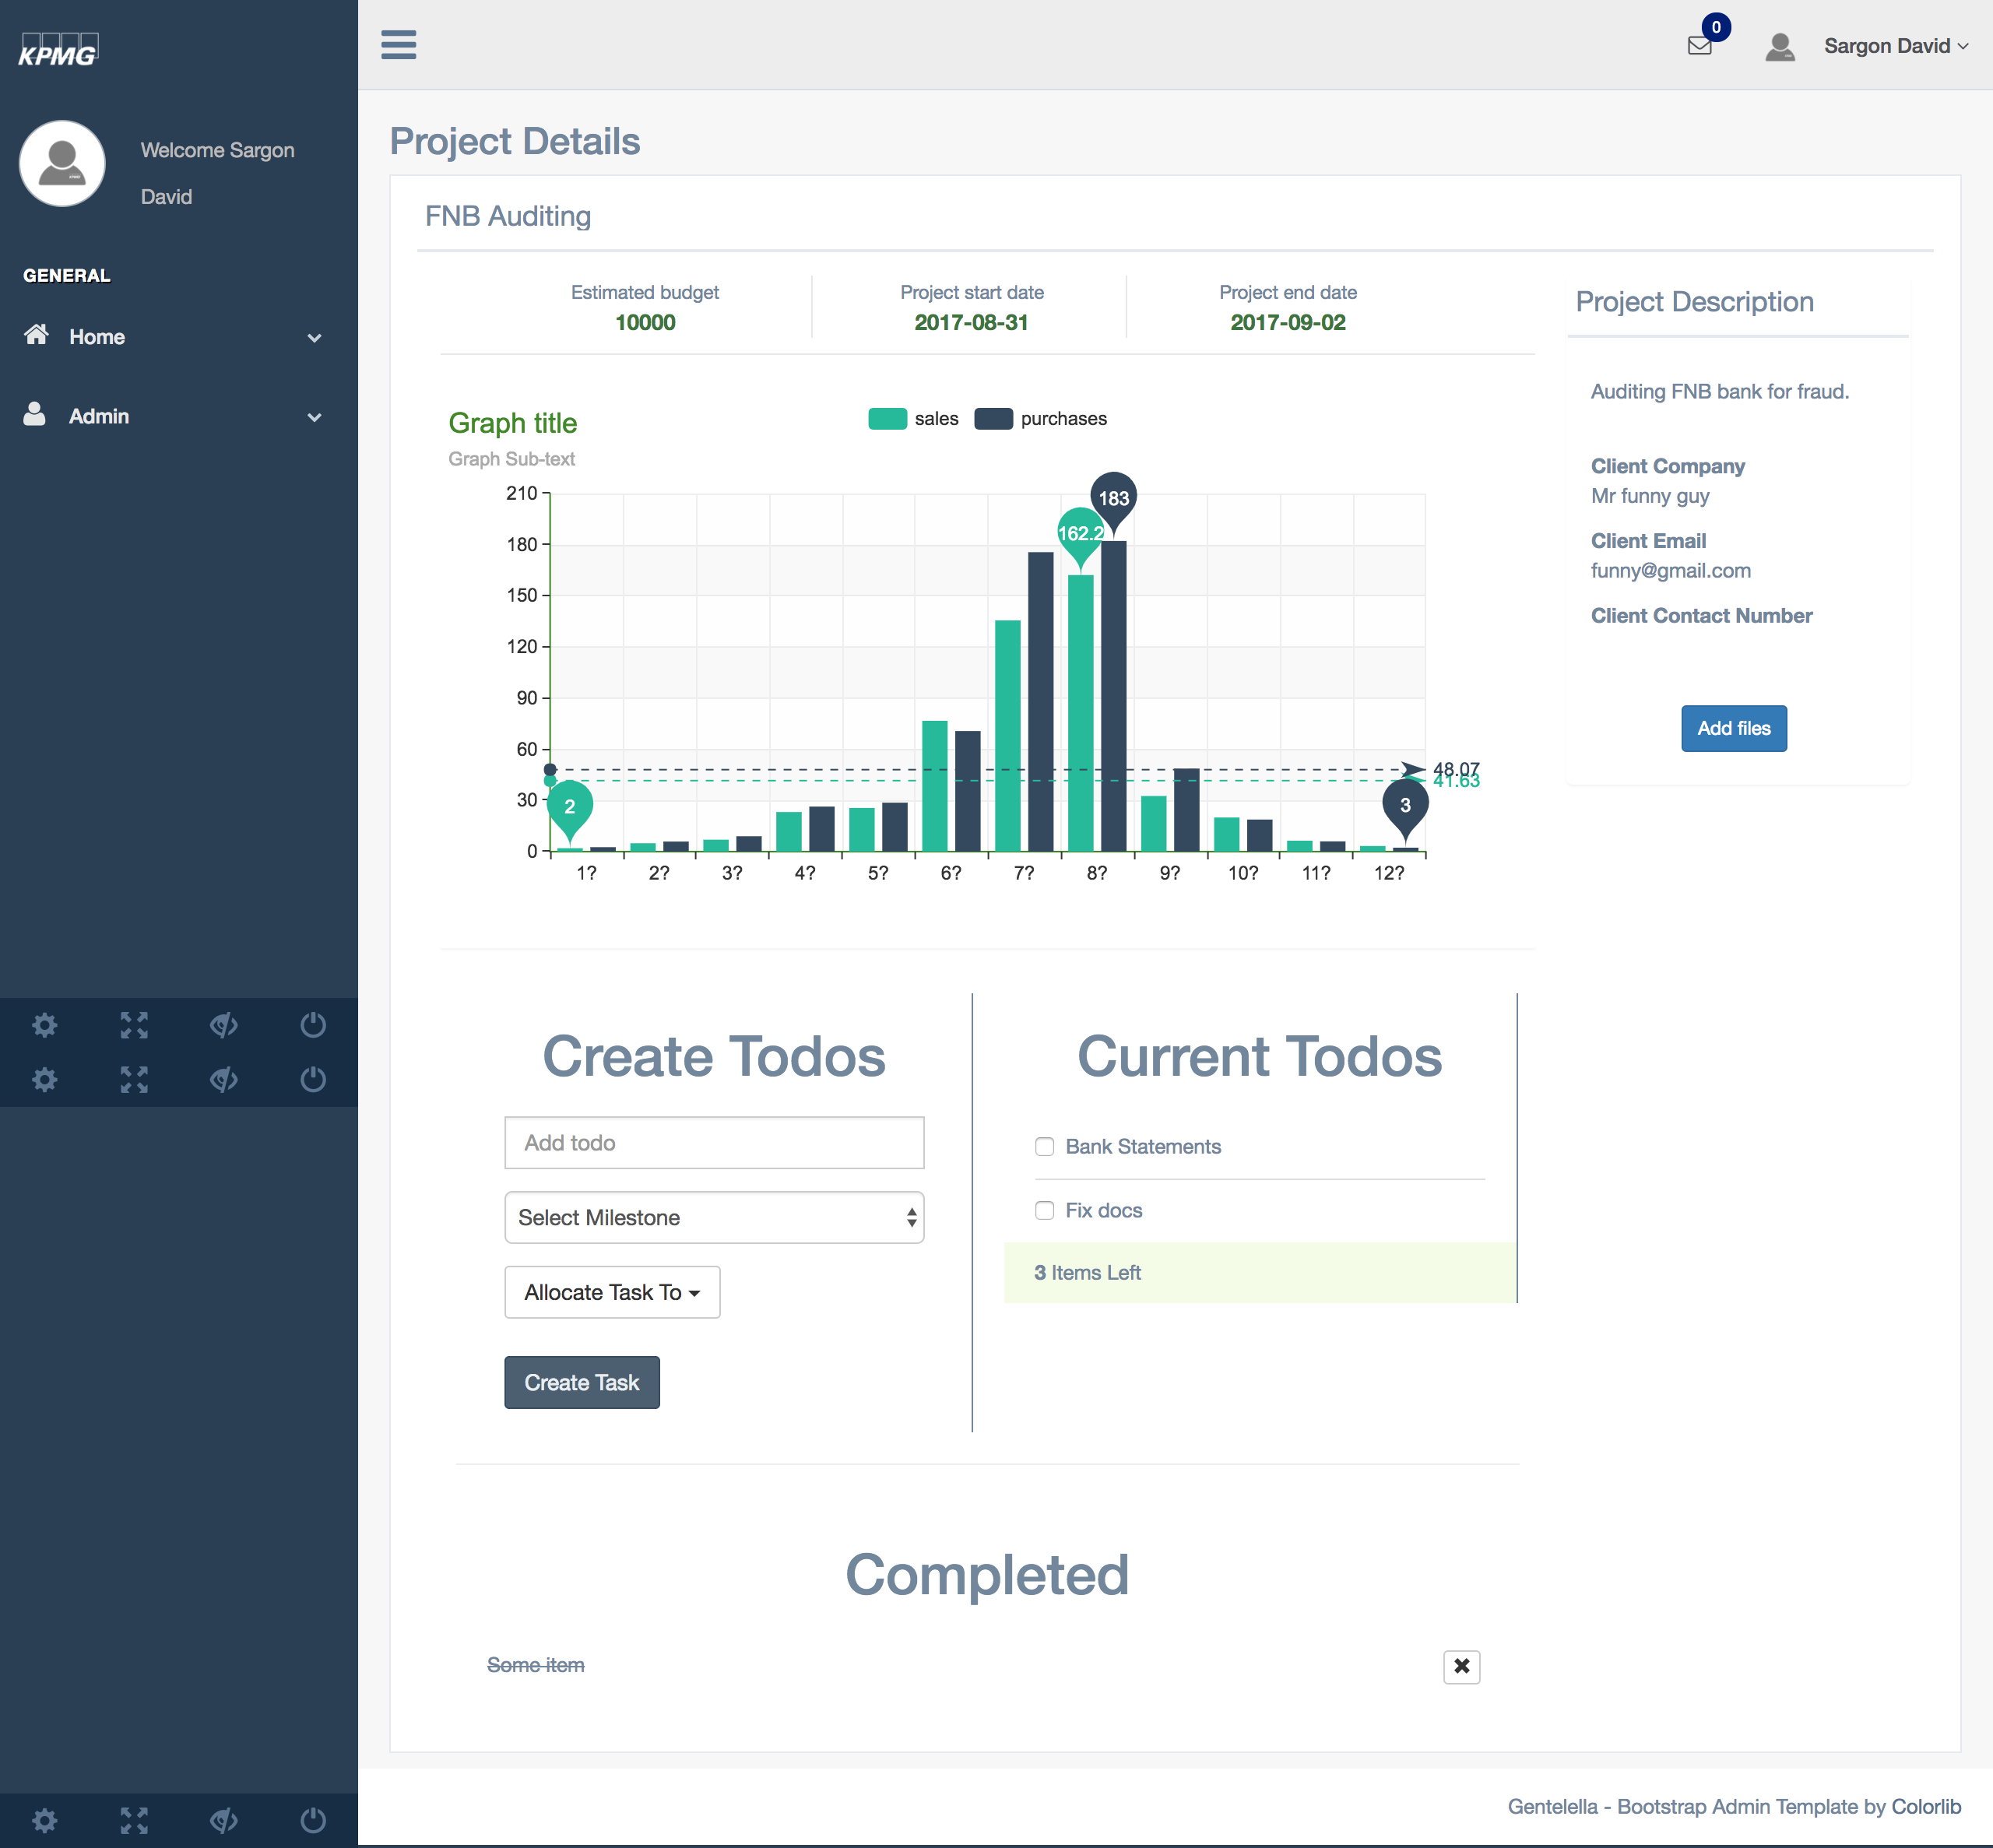
\includegraphics[width=0.99\linewidth]{Images/manager_project_detail_view.png}
				
				
		 \subsubsection{Projects Edit Page}
		 		\begin{enumerate}
				 	\item Request type: GET
				 	\item URL: \url{https://localhost:4000/project_edit}
				 \end{enumerate}
				
				\textbf{Description}
				\begin{flushright}
				  This page will allow the manager to edit the current projects deadline if needed and also remove and reassign employees if ever needed.
				\end{flushright}
				
				\textbf{Functions}
				\begin{flushright}
				    \begin{enumerate}
				    	\item  Request will be send to server that will update the project end date on the database.
				    	\item If an employee is selected to be removed, another employee of equal skill will be found. 
				     \end{enumerate}
				\end{flushright}
				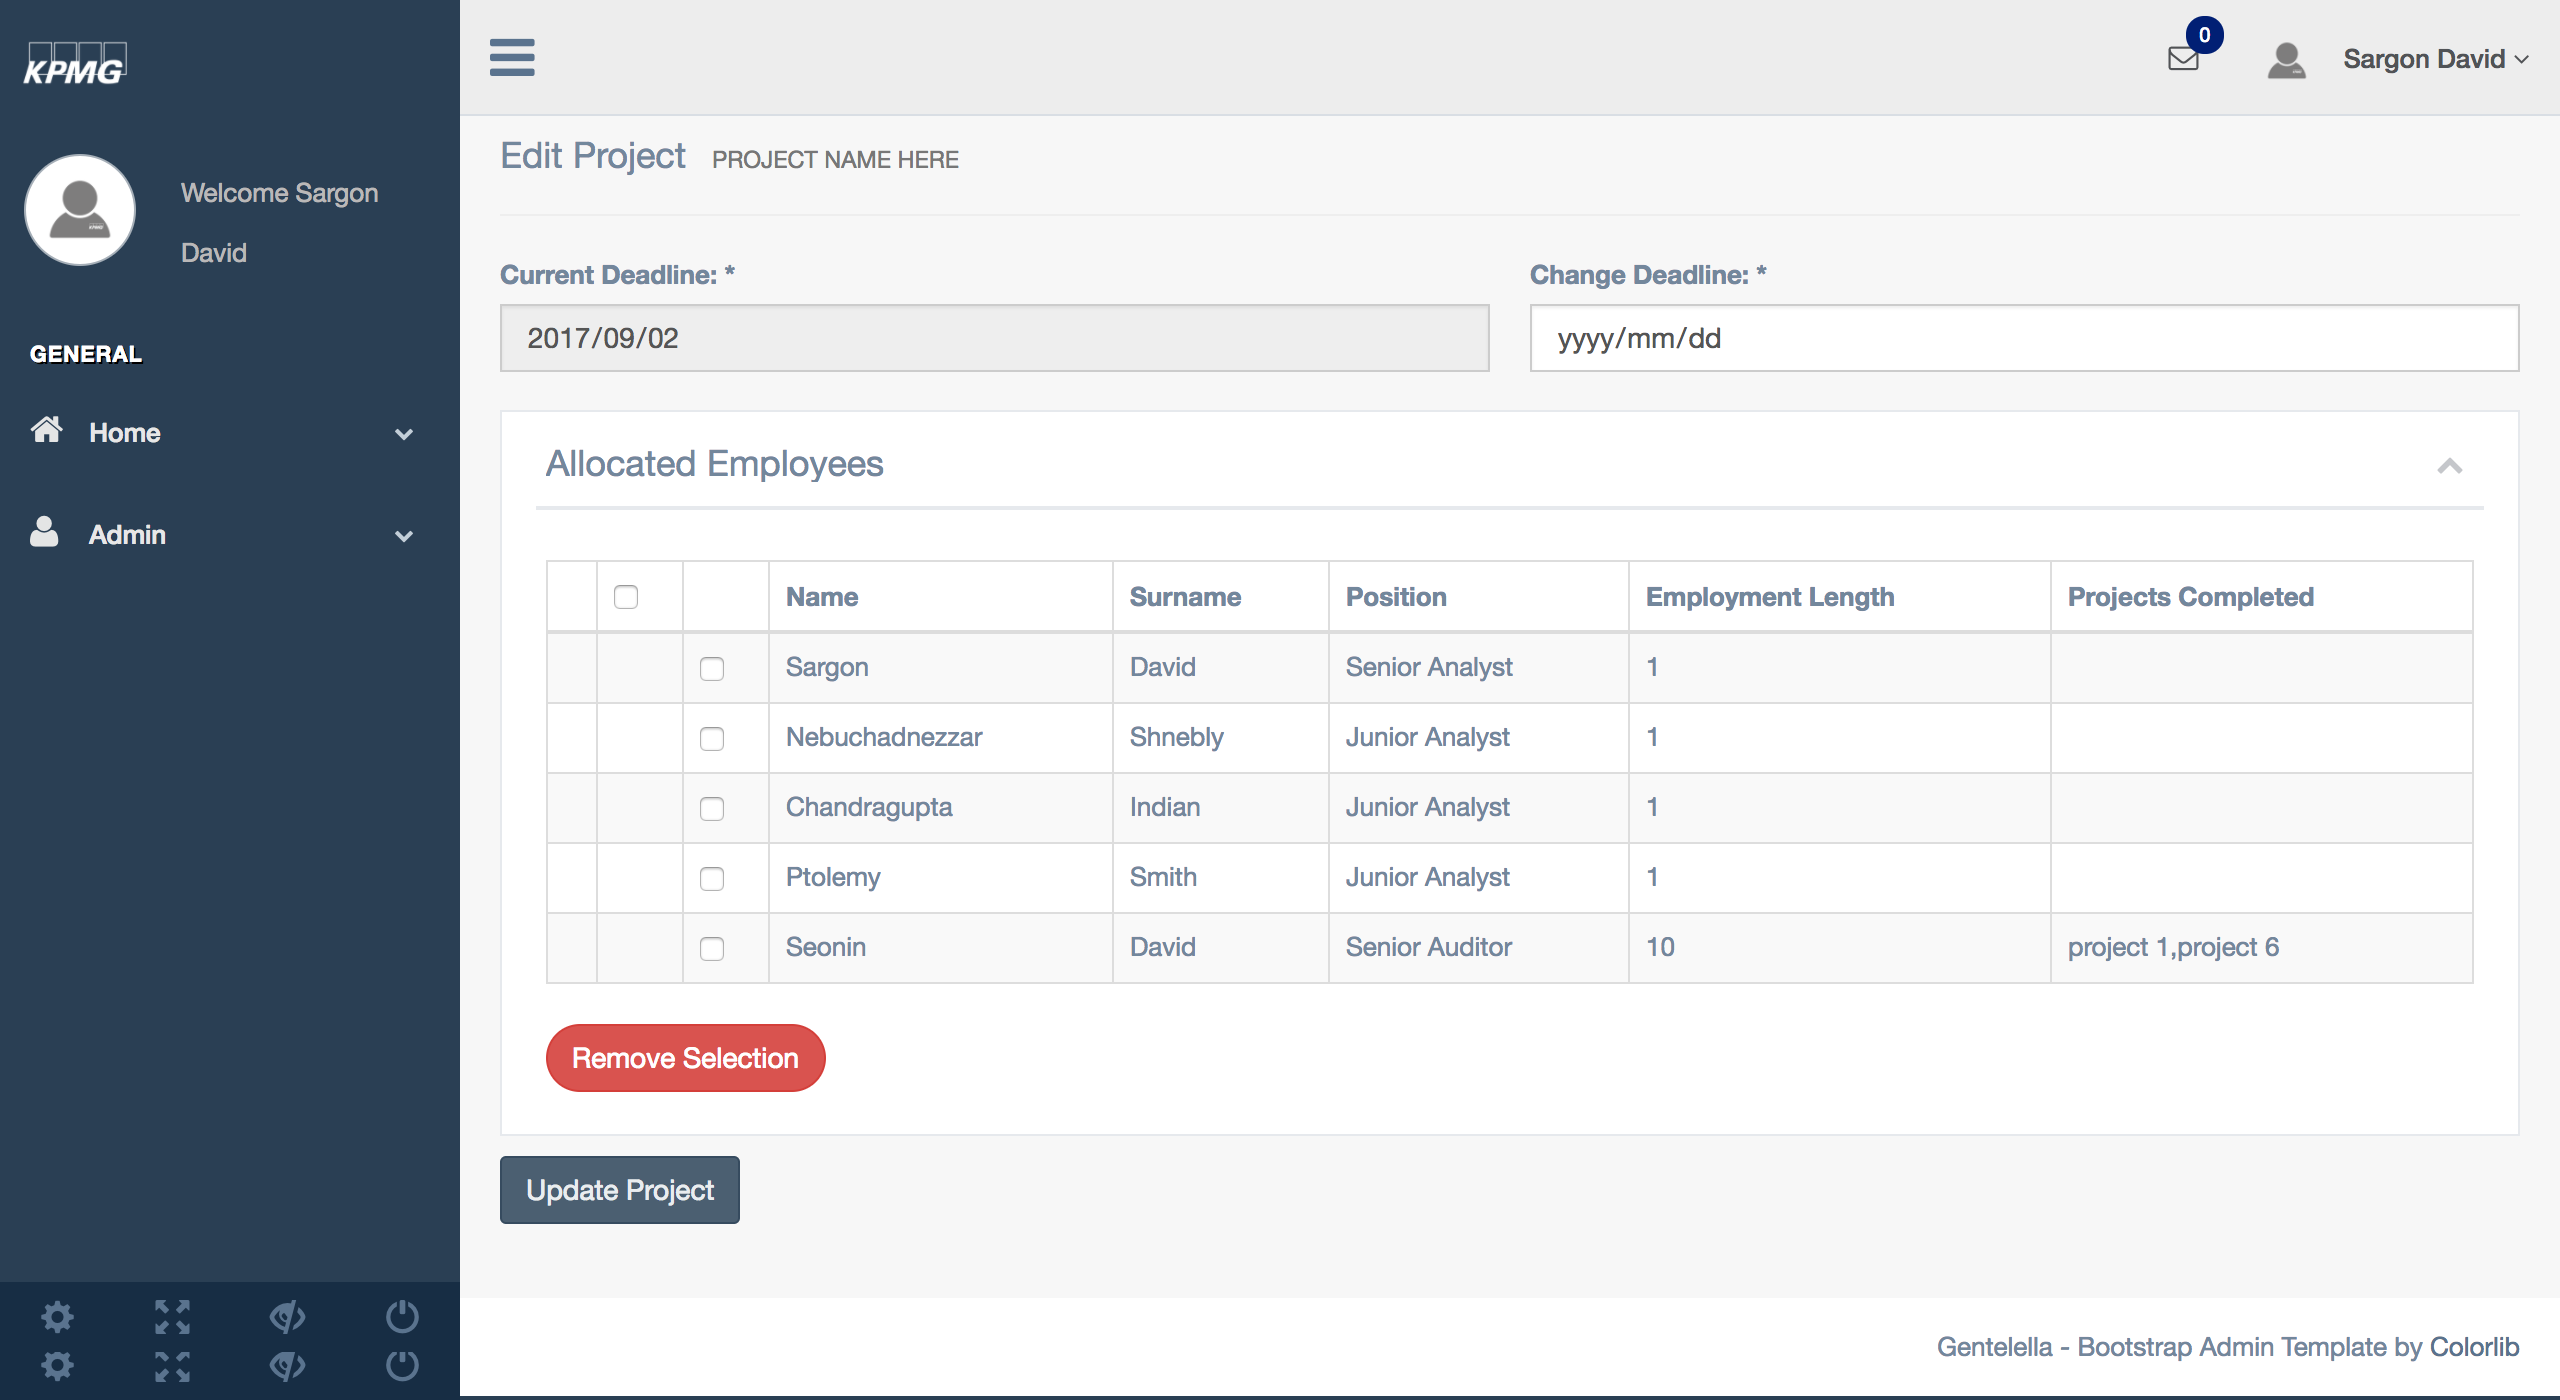
\includegraphics[width=0.99\linewidth]{Images/manager_project_edit.png}
				
		
	    \subsubsection{Milestones Page}
		 		\begin{enumerate}
				 	\item Request type: GET
				 	\item URL: \url{https://localhost:4000/project_milestone}
				 \end{enumerate}
				
				\textbf{Description}
				\begin{flushright}
				  This page will allow a project manager to create a new milestone for the project and give it the deadline date.
				\end{flushright}
				
				\textbf{Functions}
				\begin{flushright}
				    \begin{enumerate}
				    	\item Request will be sent to server to store new milestone in  database
				    	\item Now manager can assign tasks and employees to that milestone.
				     \end{enumerate}
				\end{flushright}
				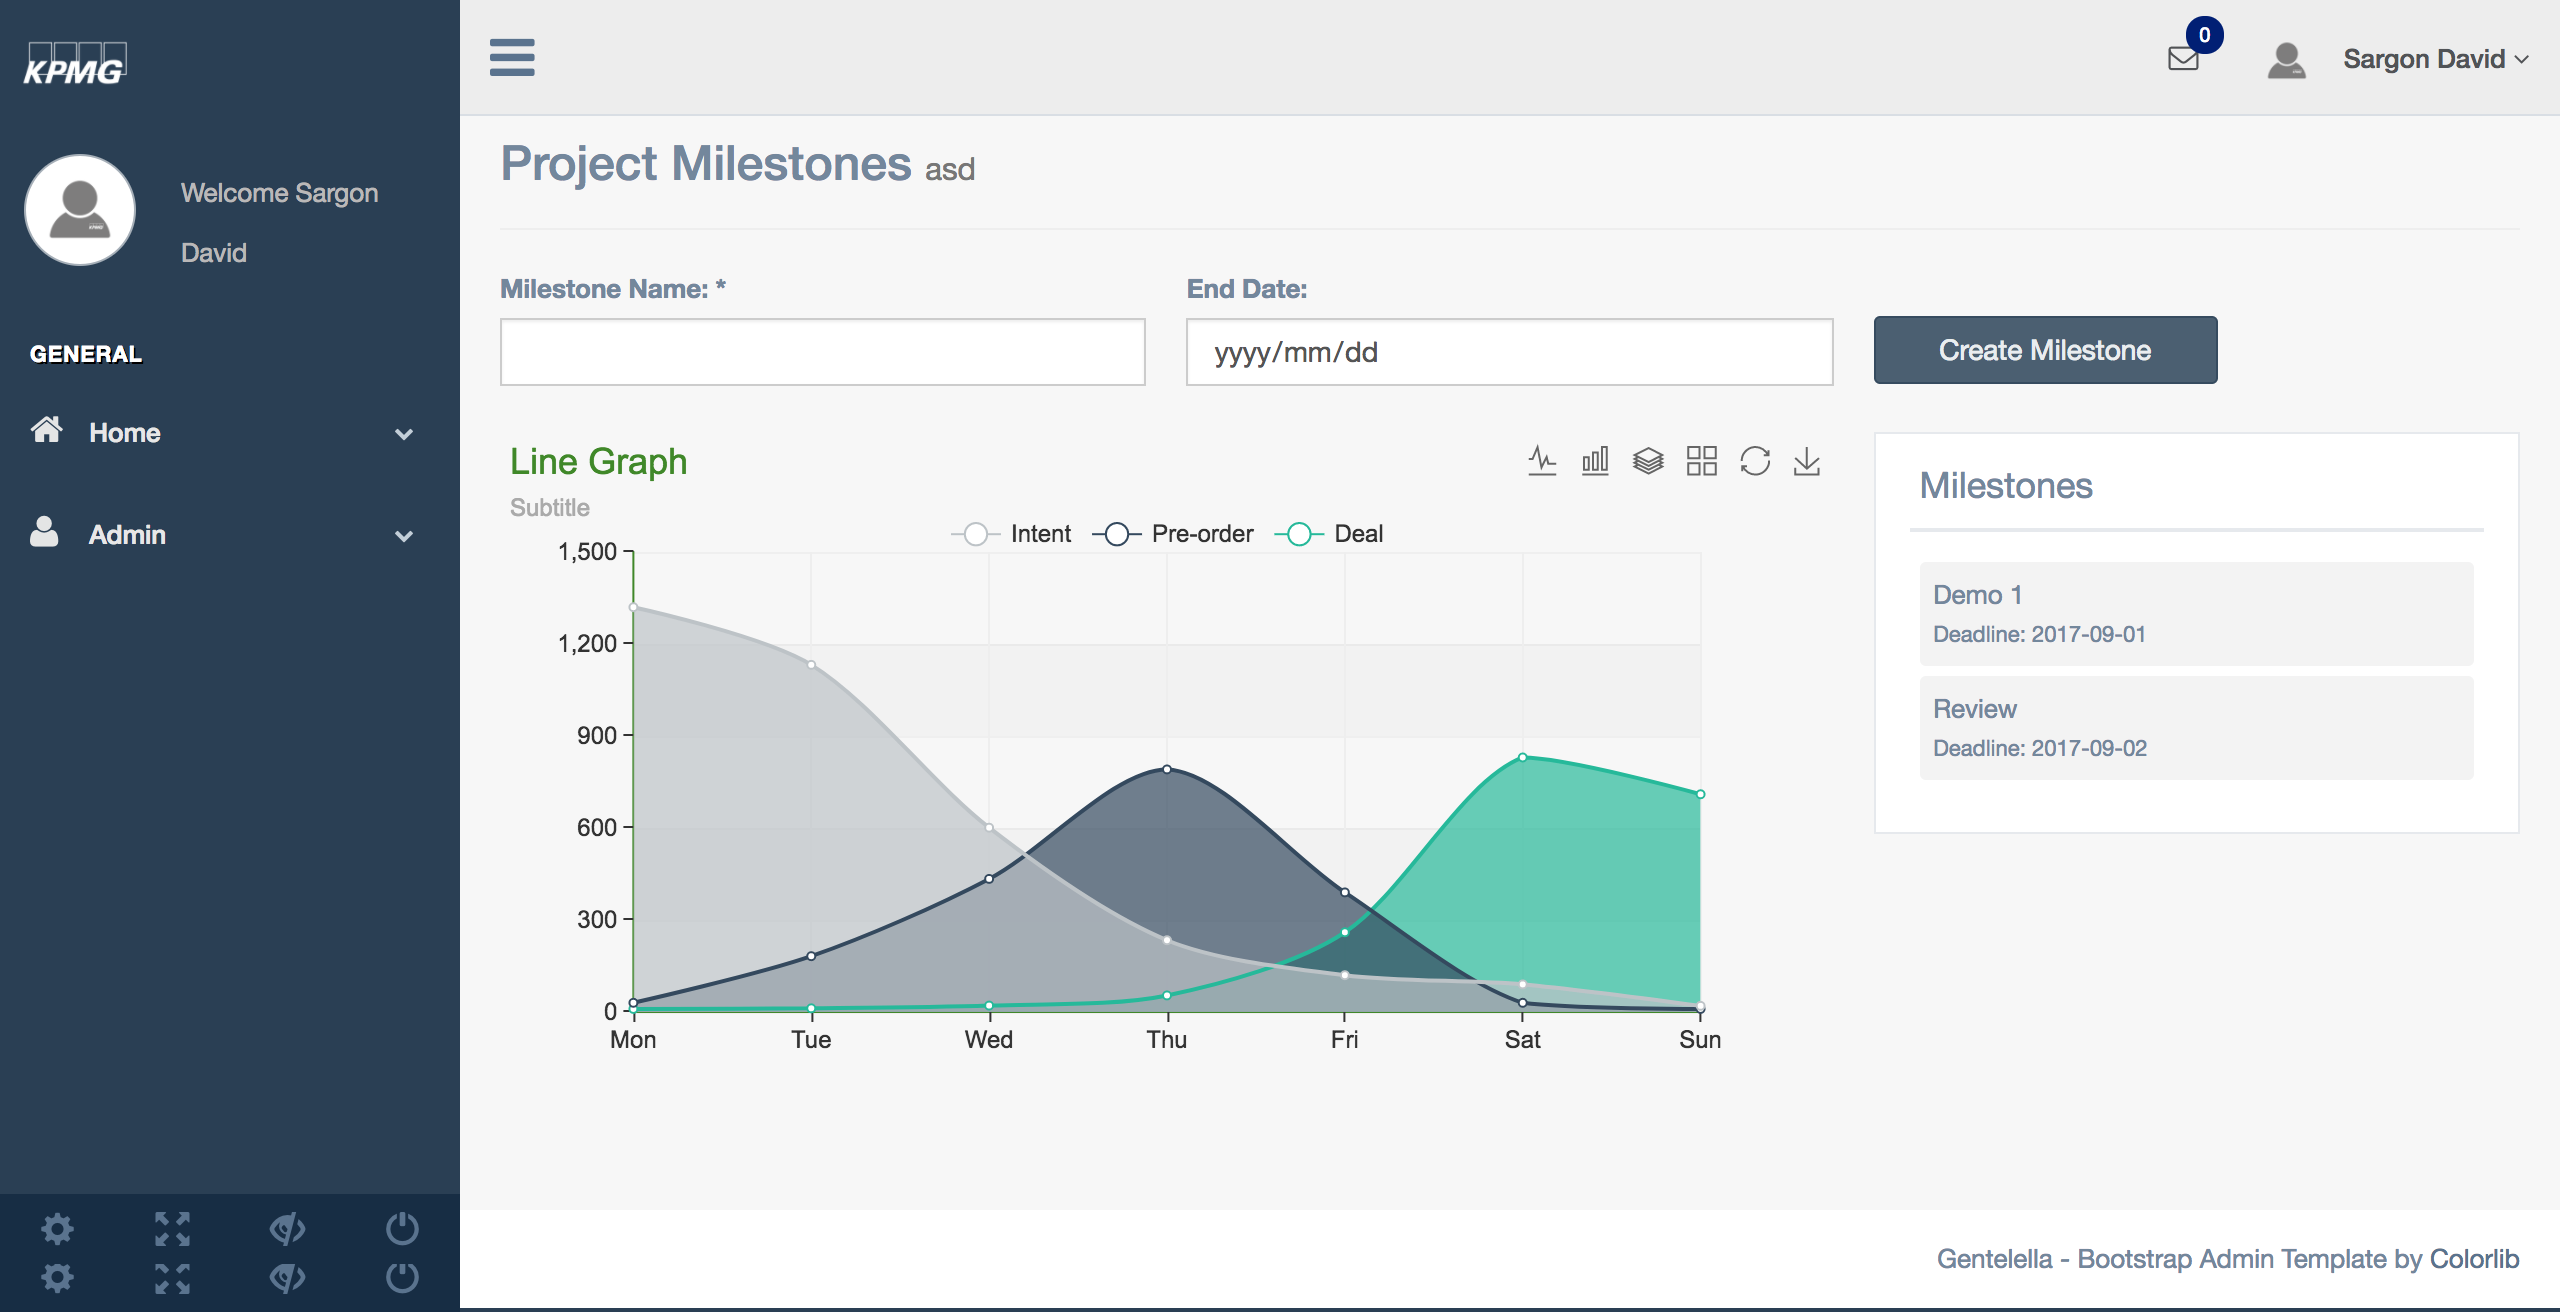
\includegraphics[width=0.99\linewidth]{Images/manager_project_milestone.png}
				
	\subsection{Employee pages (If an employee logs in)}
	     \subsubsection{Employee dashboard}
		 		\begin{enumerate}
				 	\item Request type: GET
				 	\item URL: \url{https://localhost:4000/user_dashboard}
				 \end{enumerate}
				
				\textbf{Description}
				\begin{flushright}
				  This page displays a brief overview of the employee's projects and also some analytic data regarding the current employees project.
				\end{flushright}
				
				\textbf{Functions}
				\begin{flushright}
				    \begin{enumerate}
				    	\item GET request to get the project data
				     \end{enumerate}
				\end{flushright}
				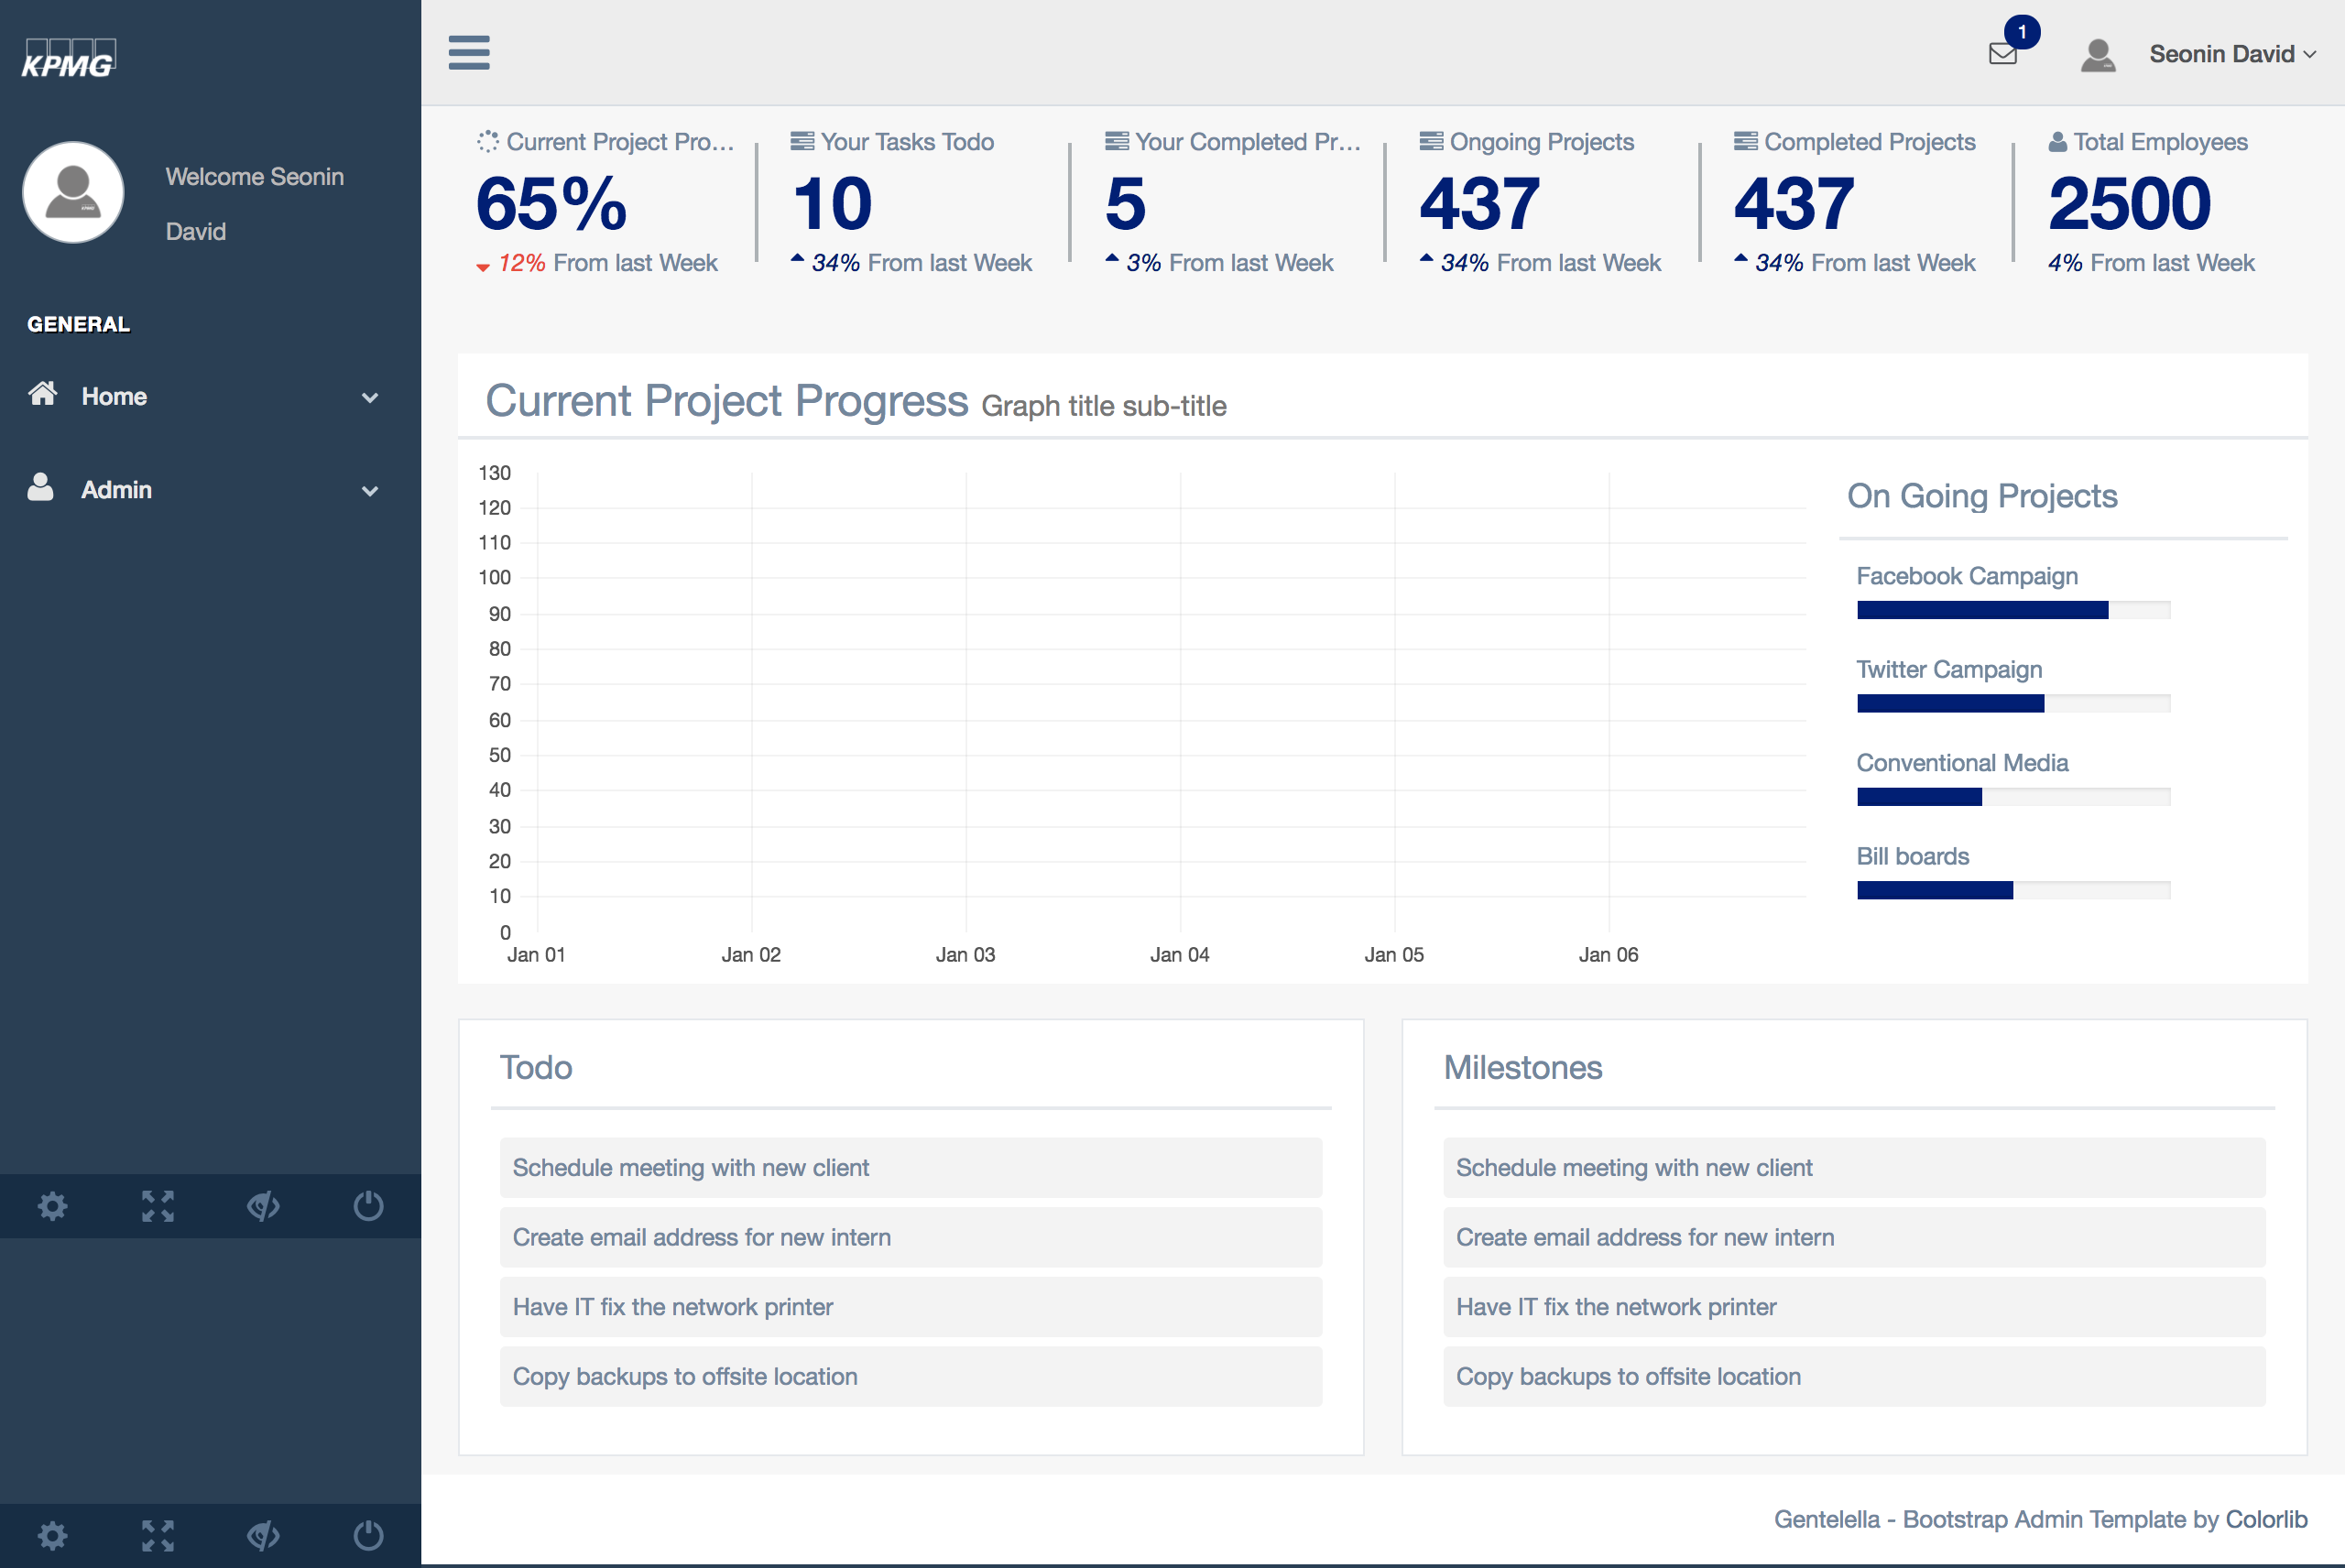
\includegraphics[width=0.99\linewidth]{Images/employee-dash.png}
				
			    \subsubsection{Employee calendar page}
		 		\begin{enumerate}
				 	\item Request type: GET
				 	\item URL: \url{https://localhost:4000/calendar}
				 \end{enumerate}
				
				\textbf{Description}
				\begin{flushright}
				 Will display all the events the employee has.Project events and personal events.
				\end{flushright}
				
				\textbf{Functions}
				\begin{flushright}
				    \begin{enumerate}
				    	\item The employee can also click on a day and create an event(as long as that event does not conflict with the project.)
				     \end{enumerate}
				\end{flushright}
				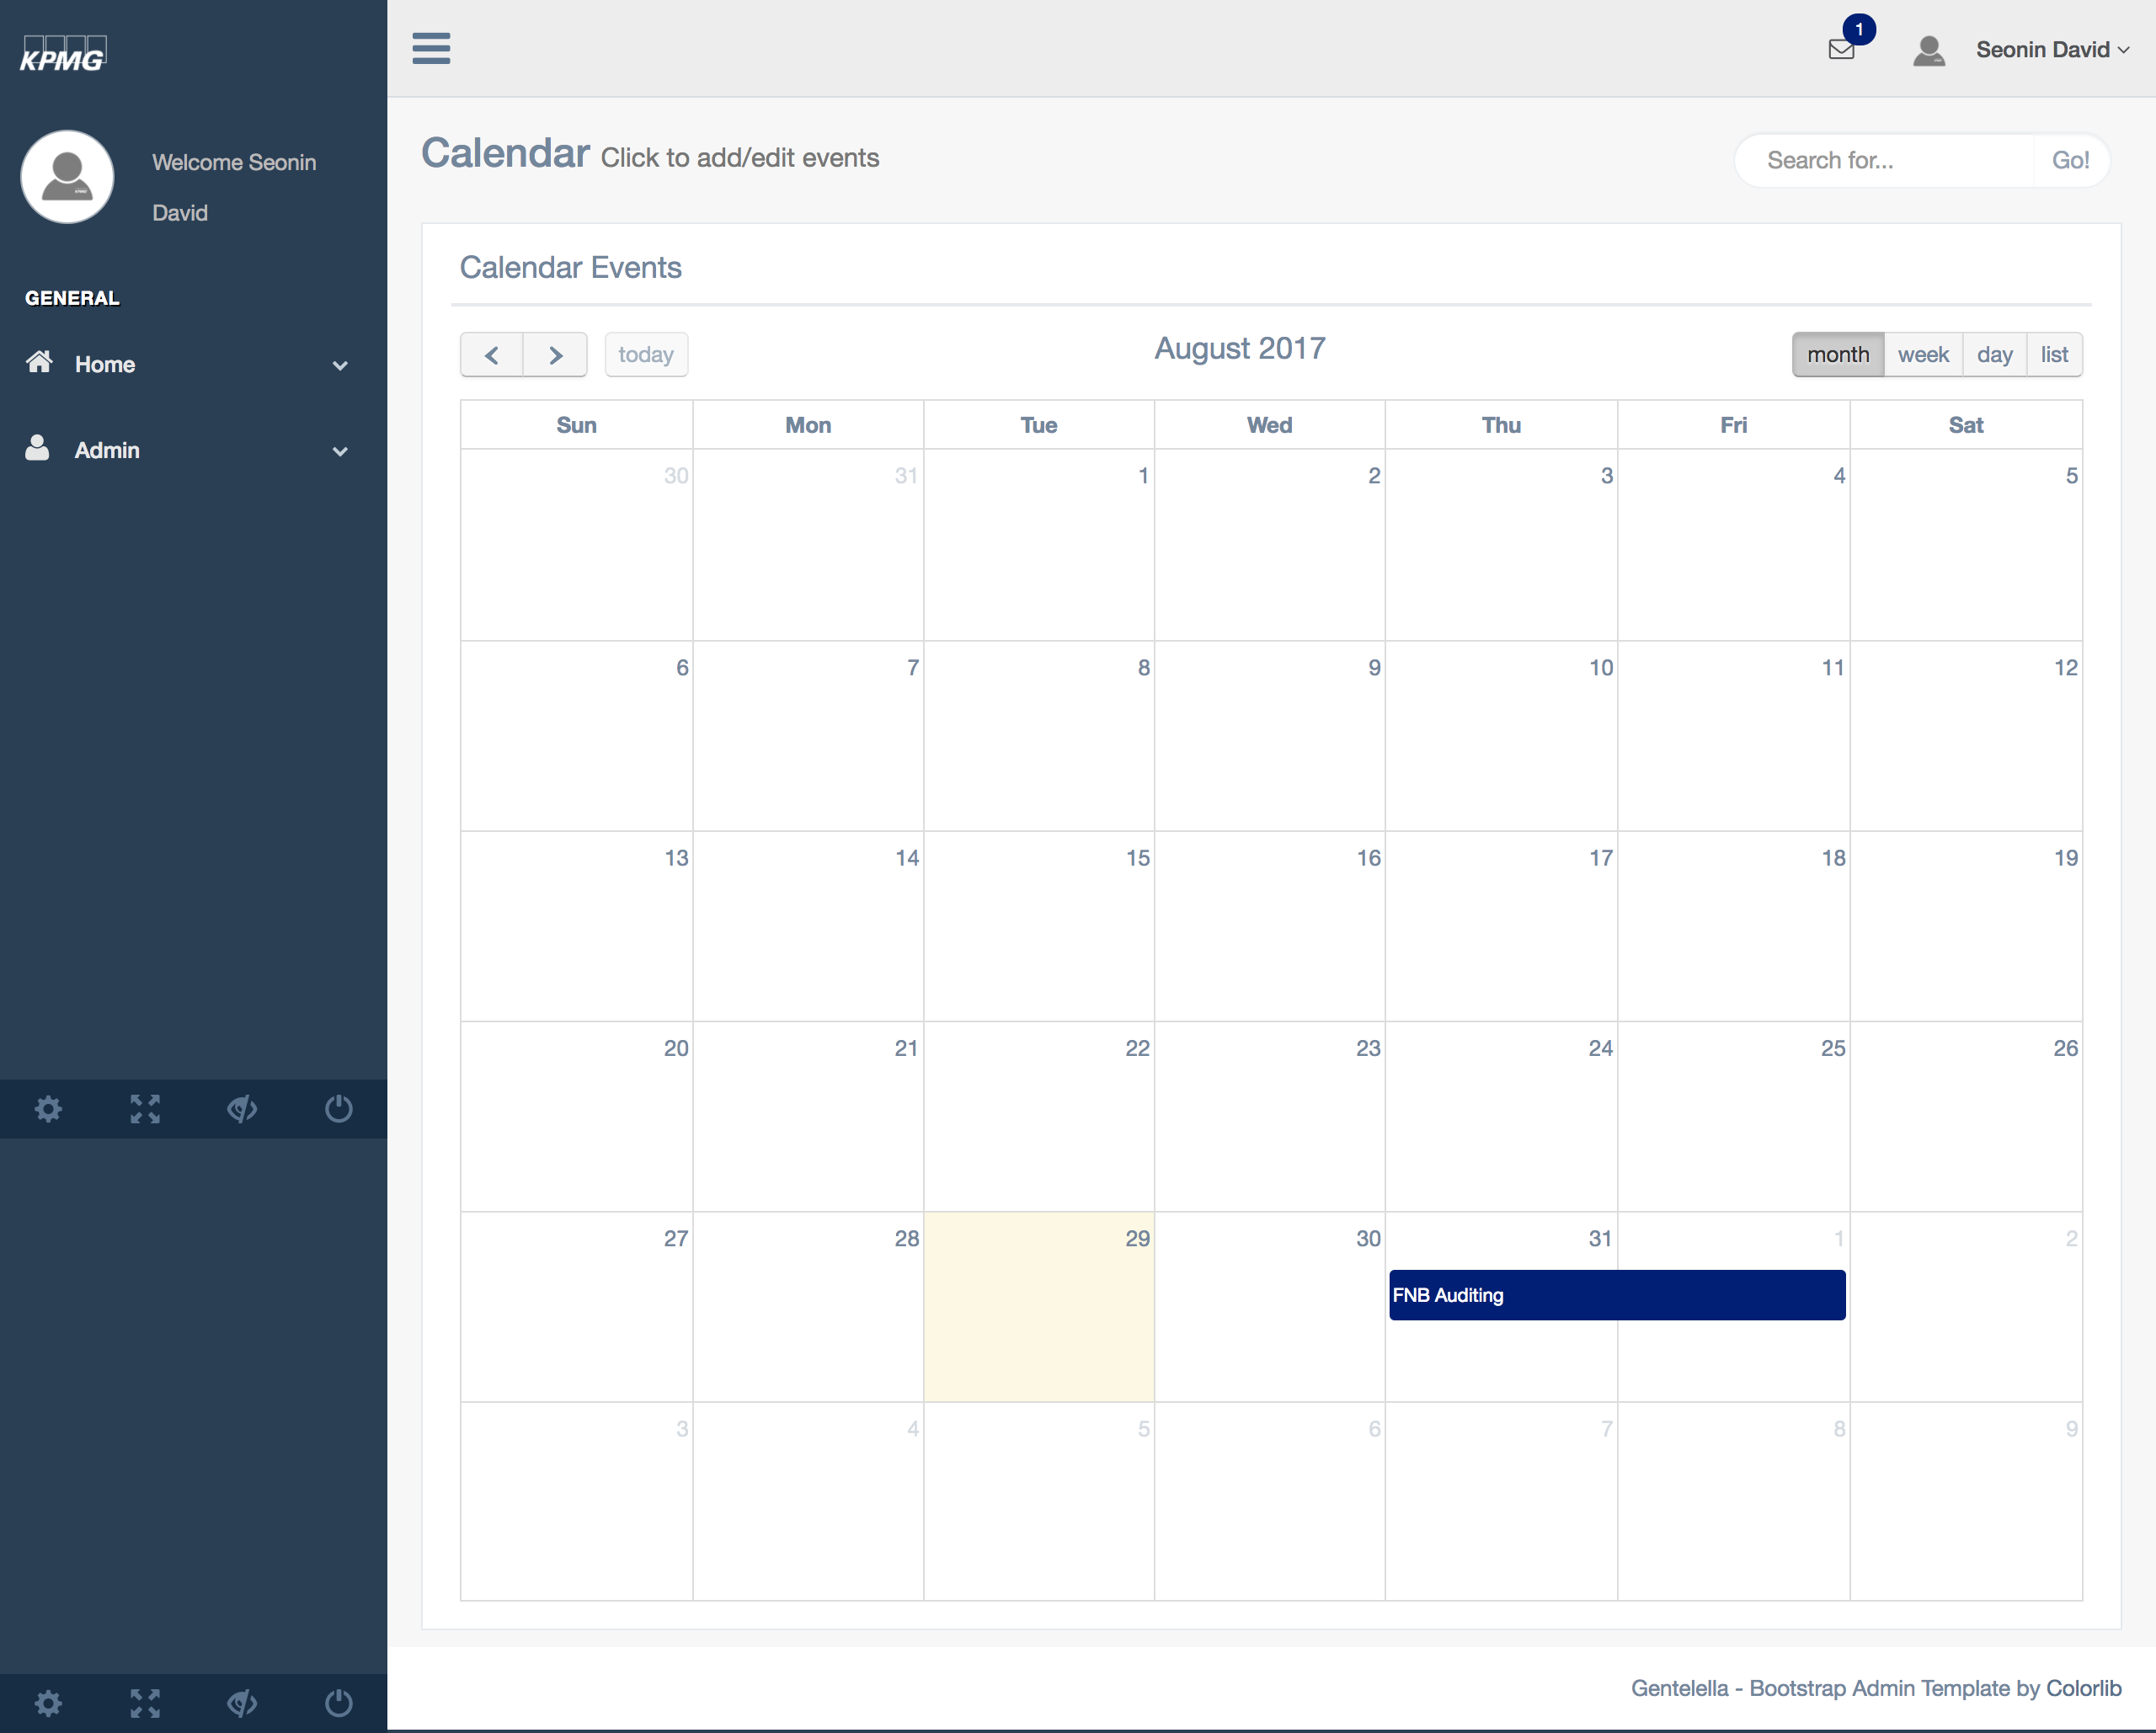
\includegraphics[width=0.99\linewidth]{Images/employee_calendar.png}
				
				
\end{document}
